\documentclass[10pt,preprint]{aastex}

\usepackage{amsfonts}
\usepackage{amsmath}
\usepackage{amssymb}
\usepackage{amsthm}
\usepackage{booktabs}
\usepackage{mathrsfs}
\usepackage{cite}
\usepackage{times}
\usepackage{url}
\usepackage{hyperref}
\usepackage{lineno}
\usepackage{yhmath}
\usepackage{natbib}
\usepackage{../definitions}
\hypersetup{
  bookmarksnumbered = true,
  bookmarksopen=false,
  pdfborder=0 0 0,         % make all links invisible, so the pdf looks good when printed
  pdffitwindow=true,      % window fit to page when opened
  pdfnewwindow=true, % links in new window
  colorlinks=true,           % false: boxed links; true: colored links
  linkcolor=blue,            % color of internal links
  citecolor=magenta,    % color of links to bibliography
  filecolor=magenta,     % color of file links
  urlcolor=cyan              % color of external links
}

\newcommand{\ee}[1]{{\color{red} #1}}
\newcommand{\dx}{\Delta x}
\newcommand{\pbK}{\partial\mathbf{K}}
\newcommand{\UDG}{\bU_{\mbox{\tiny DG}}}
\newcommand{\sumx}{\sum_{i=1}^{d}}
\newcommand{\NES}{\mbox{\tiny NES}}

\begin{document}

\title{Nodal Discontinuous Galerkin Method for the Two-Moment Model of Neutrino Transport}
\author{Eirik Endeve\altaffilmark{1}, et al.}
\altaffiltext{1}{Computational and Applied Mathematics Group, Oak Ridge National Laboratory, Oak Ridge, TN 37831-6354, USA; endevee@ornl.gov}

\begin{abstract}
We present a nodal Discontinuous Galerkin (DG) method for solving the non-relativistic two-moment model for neutrino transport.  
The method --- ultimately targeted for simulations of core-collapse supernovae --- includes the use of curvilinear coordinates and non-ideal microphysics (nuclear equation of state and weak interactions) for neutrino-matter interactions.  
\end{abstract}

\tableofcontents

\section{Introduction}

We will use inits in which the speed of light is unity ($c=1$).  

\section{Two-Moment Model for Neutrino Transport}

\subsection{Basic Mathematical Model}

For general curvilinear spatial coordinates $\{x^{i}\}$, the two-moment model for radiation transport takes the form \citep[see, e.g.,][for fully general relativistic treatments]{shibata_etal_2011,cardall_etal_2013a}
\begin{align}
  &\f{1}{\sqrt{\gamma}}\pderiv{}{t}\Big(\,\sqrt{\gamma}\,\cJ\,\Big)
  +\f{1}{\sqrt{\gamma}}\pderiv{}{x^{i}}\Big(\,\sqrt{\gamma}\,\cH^{i}\,\Big)
  =\tilde{\chi}\,\big(\cJ_{0}-\cJ\big) \nonumber \\
  &\hspace{12pt}
  +\big(4\pi-\cJ\big)\int_{\bbR^{+}}R^{\In}(\epsilonNu,\epsilonNu')\,\cJ(\epsilonNu')\,dV_{\epsilonNu'}
  -\cJ\int_{\bbR^{+}}R^{\Out}(\epsilonNu,\epsilonNu')\,\big(4\pi-\cJ(\epsilonNu')\big)\,dV_{\epsilonNu'},
  \label{eq:momentEquationEnergy}
\end{align}
\begin{align}
  &\f{1}{\sqrt{\gamma}}\pderiv{}{t}\Big(\,\sqrt{\gamma}\,\cH_{j}\,\Big)
  +\f{1}{\sqrt{\gamma}}\pderiv{}{x^{i}}\Big(\,\sqrt{\gamma}\,\cK^{i}_{~j}\,\Big)
  =\f{1}{2}\,\cK^{ik}\,\pderiv{\gamma_{ik}}{x^{j}}-\kappa\,\cH_{j} \nonumber \\
  &\hspace{12pt}
  -\cH_{j}\int_{\bbR^{+}}\big[\,R^{\In}(\epsilonNu,\epsilonNu')\,\cJ(\epsilonNu')+R^{\Out}(\epsilonNu,\epsilonNu')\big(4\pi-\cJ(\epsilonNu')\big)\,\big]\,dV_{\epsilonNu'},
  \label{eq:momentEquationMomentum}
\end{align}
where $\cJ$, $\cH^{i}$, and $\cK^{ij}$ are defined as angular moments of a positive neutrino distribution function $f(\omegaNu,\epsilonNu,\bx,t)$
\begin{equation}
  \big\{\,\cJ,\,\cH^{i},\,\cK^{ij}\,\big\}(\epsilonNu,\bx,t)
  =\int_{\bbS^{2}}f(\omegaNu,\epsilonNu,\bx,t)\,\big\{1,l^{i},l^{i}\,l^{j}\}\,d\omegaNu.  
  \label{eq:angularMoments}
\end{equation}
Here, $\{l^{i}\}$ are components of a unit three-vector proportional to the neutrino three-momentum $\bp=\epsilonNu\,\bl$.  
(We adopt the Einstein summation convention and let repeated Latin indices run from $1$ to $3$.)
In a kinetic description, neutrinos are described by the phase space distribution function $f$, and the momentum space coordinates used here are the neutrino energy $\epsilonNu$, and the angles $\thetaNu$ and $\phiNu$ (describing the neutrino propagation direction relative to a local orthonormal basis).  
In forming the angular moments in Eq.~\eqref{eq:angularMoments}, the integrals extend over the unit sphere
\begin{equation}
  \bbS^{2}=\big\{\,(\thetaNu,\phiNu)~|~\thetaNu\in[0,\pi),\,\phiNu\in[0,2\pi)\,\big\}.  
\end{equation}
The angular moments are related to the neutrino energy density, momentum density, and stress ($\cJ$, $\cH^{i}$, and $\cK^{ij}$, respectively).  
They are functions of the neutrino energy $\epsilonNu$, spatial position $\{x^{i}\}$, and time $t$.  

To model neutrino matter interactions, we include emission and absorption, (isotropic) elastic scattering on nucleons and nuclei, and neutrino-electron scattering (NES).  
On the right-hand sides of Eqs.~\eqref{eq:momentEquationEnergy} and \eqref{eq:momentEquationMomentum}, $\tilde{\chi}(\epsilonNu,\bU)$ and $\kappa(\epsilonNu,\bU)=\tilde{\chi}(\epsilonNu,\bU)+\sigma(\epsilonNu,\bU)$ are absorption and total (absorption plus scattering) opacities, respectively.  
The absorption opacity $\tilde{\chi}$ is corrected for stimulated absorption \citep[cf.][]{mezzacappaBruenn_1993a}.  
The NES rates $R^{\In}$ and $R^{\Out}$ are obtained by expanding the full kernels in a Legendre series, retaining only the isotropic part \citep[see, e.g.,][]{cernohorsky_1994}, and the integrals extend over all energies $\bbR^{+}=\{\epsilonNu~|~\epsilonNu\in[0,\infty)\}$.  
The energy volume element is $dV_{\epsilonNu}=\epsilonNu^{2}d\epsilonNu$.  
The opacities depend on the neutrino energy and the local thermodynamic state of the fluid $\bU=(\rho,T,Y_{e})^{T}$, where $\rho$ is the (baryon) mass density, $T$ the temperature, and $Y_{e}$ the electron fraction.  
For simplicity we consider a single neutrino species (electron neutrinos), and we use opacities given by \citet{bruenn_1985}; see Section~\ref{sec:opacities} for further details.  
In Eq.~\eqref{eq:momentEquationEnergy}, the equilibrium density $\cJ_{0}=4\pi\,f_{0}(\epsilonNu,\bU)$ is computed from the angular moment of the isotropic Fermi-Dirac distribution
\begin{equation}
  f_{0}(\epsilonNu,\bU)=\f{1}{e^{(\epsilonNu-\mu_{\nu})/k_{\mbox{\tiny B}}T}+1},
\end{equation}
where $k_{\mbox{\tiny B}}$ is Boltzmann's constant, and $\mu_{\nu}=\mu_{p}-\mu_{n}+\mu_{e}$ is the neutrino chemical potential.  
(The chemical potentials of protons, neutrons, and electrons are denoted by $\mu_{p}$, $\mu_{n}$, and $\mu_{e}$, respectively.)

The model given by Eqs.~\eqref{eq:momentEquationEnergy} and \eqref{eq:momentEquationMomentum} is non-relativistic (i.e., it does not include effects due to strong gravitational fields or interactions with a moving fluid), but is expressed in terms of curvilinear coordinates through the spatial metric tensor $\gamma_{ij}$, which gives squared infinitesimal line-element
\begin{equation}
  ds_{\vect{x}}^{2}=\gamma_{ij}\,dx^{i}\,dx^{j},
\end{equation}
where $\gamma_{ij}$ are the spatial components of the coordinate basis metric tensor.  
We will make two simplifying assumptions: the metric tensor is (1) diagonal and (2) time-independent.  
Specifically we assume the following diagonal form
\begin{equation}
  \gamma_{ij}
  =\mbox{diag}\big[\,\gamma_{11},\,\gamma_{22}(x^{1}),\,\gamma_{33}(x^{1},x^{2})\,\big], 
  \label{eq:threeMetric}
\end{equation}
which is sufficiently general to accommodate Cartesian, cylindrical, and spherical polar coordinates (see Table~\ref{tab:metricFunctions} and Appendix~\ref{app:CurvilinearEuler}).  
Moreover, $\gamma$ is the determinant of the metric tensor, and $\sqrt{\gamma}=\sqrt{\gamma_{11}\gamma_{22}\gamma_{33}}$.  
The inverse of the spatial metric is denoted $\gamma^{ij}$, so that $\gamma^{ik}\gamma_{kj}=\delta^{i}_{~j}$.  
We can use the spatial metric to raise and lower indices on spatial vectors and tensors; e.g., $\cH_{j}=\gamma_{jk}\,\cH^{k}$.  

The two-moment system contains the higher order moments $\cK^{ij}$ --- the symmetric stress tensor.  
In order to form a closed system of equations, the components of the stress tensor must be related to the lower order moments through a closure procedure.  
Following \citet{levermore_1984}, we write
\begin{equation}
  \cK^{i}_{~j}
  =\f{1}{2}\,\Big[\,(1-\psi)\,\delta^{i}_{~j}+(3\,\psi-1)\,h^{i}\,h_{j}\,\Big]\,\cJ,
  \label{eq:stressTensor}
\end{equation}
where $\psi$ is the Eddington factor, $h^{i}=\cH^{i}/\cH$, and $\cH=\sqrt{\cH_{i}\cH^{i}}$.  
We also define the flux factor $h=\cH/\cJ$, and use the analytic expression for the Eddington factor \citep{minerbo_1978} given by 
\begin{equation}
  \psi(h)=\f{1}{3}+\f{2}{3}\,\Big(\,h^{2}\,\big(\,3-h+3h^{2}\,\big)/5\,\Big),
  \label{eq:eddingtonFactor}
\end{equation}
which approximates the low occupancy limit of the maximum entropy closure for Fermi-Dirac particles given by \citet{cernohorskyBludman_1994}.  
Specifically, we have $\psi(0)=1/3$ (diffusion limit) and $\psi(1)=1$ (streaming limit).  

\subsection{Two-Moment Model as a System of Conservation Laws with Sources}

\begin{table}
  \begin{center}
  \caption{Relevant metric functions for Cartesian, Cylindrical, and Spherical coordinate systems.\label{tab:metricFunctions}}
  \begin{tabular}{ccccccccccc}
    \midrule
    Coordinates & $x^{1}$ & $x^{2}$ & $x^{3}$ & $\gamma_{11}$ & $\gamma_{22}$ & $\gamma_{33}$ & $\sqrt{\gamma}$
    & $\f{1}{\gamma_{22}}\pderiv{\gamma_{22}}{x^{1}}$ & $\f{1}{\gamma_{33}}\pderiv{\gamma_{33}}{x^{1}}$ & $\f{1}{\gamma_{33}}\pderiv{\gamma_{33}}{x^{2}}$ \\
    \midrule
    \midrule
    Cartesian & $x$ & $y$ & $z$ & 1 & 1 & 1 & 1 & 0 & 0 & 0 \\
    Cylindrical & $R$ & $z$ & $\phi$ & 1 & 1 & $R^{2}$ & $R$ & 0 & $2/R$ & 0 \\
    Spherical & $r$ & $\theta$ & $\phi$ & 1 & $r^{2}$ & $r^{2}\sin^{2}\theta$ & $r^{2}\sin\theta$ & $2/r$ & $2/r$ & $2\cot\theta$ \\
    \midrule
    \midrule
  \end{tabular}
  \end{center}
\end{table}

For the forthcoming description it is useful to write the moment equations in a more compact form.  
To this end, we define the geometry sources in Eq.~\eqref{eq:momentEquationMomentum} by
\begin{equation}
  \cG_{j}
  =\f{1}{2}\,\cK^{ik}\,\pderiv{\gamma_{ik}}{x^{j}}.  
\end{equation}
Specifically, using the time-independent metric tensor in Eq.~\eqref{eq:threeMetric} and writing in terms of $\cK^{i}_{~j}$, the components are
\begin{equation}
  \cG_{1}
  =\f{1}{2}\,\Big(\,\cK^{2}_{~2}\,\f{1}{\gamma_{22}}\pderiv{\gamma_{22}}{x^{1}}+\cK^{3}_{~3}\,\f{1}{\gamma_{33}}\pderiv{\gamma_{33}}{x^{1}}\,\Big), \quad
  \cG_{2}
  =\f{1}{2}\,\cK^{3}_{~3}\,\f{1}{\gamma_{33}}\pderiv{\gamma_{33}}{x^{2}}, \quad\text{and}\quad
  \cG_{3}
  =0.
\end{equation}
(Explicit expressions for metric functions appearing in the geometry sources are listed in Table~\ref{tab:metricFunctions}.)  
Then, by defining the vector of evolved moments $\bcM=\big(\,\cJ,\,\bcH\,\big)^{T}$, the vector of geometry sources $\bcG(\bcM)=\big(\,0,\,\cG_{1},\,\cG_{2},\,\cG_{3}\,\big)^{T}$, the vector of collision sources $\bcC(\bcM)=\big(\,\chi\,(\cJ_{0}-\cJ)+\cL_{\NES},\,-(\kappa+\kappa_{\NES})\,\bcH\,\big)^{T}$, and the flux vectors $\bcF^{i}(\bcM)=\big(\,\cH^{i},\,\cK_{~1}^{i},\,\cK_{~2}^{i},\,\cK_{~3}^{i}\,\big)^{T}$, we write the system of equations in compact form
\begin{equation}
  \f{1}{\sqrt{\gamma}}\pderiv{}{t}\Big(\,\sqrt{\gamma}\,\bcM\,\Big)
  +\f{1}{\sqrt{\gamma}}\pderiv{}{x^{i}}\Big(\,\sqrt{\gamma}\,\bcF^{i}(\bcM)\,\Big)
  =\bcG(\bcM)+\bcC(\bcM).
  \label{eq:momentEquationsCompact}
\end{equation}
Here, $\cL_{\NES}$ and $\kappa_{\NES}$ represent the integral operators appearing in Eqs.~\eqref{eq:momentEquationEnergy} and \eqref{eq:momentEquationMomentum}, respectively.  
Eq.~\eqref{eq:momentEquationsCompact} forms the basis for developing DG methods for neutrino transport.  

\section{Discontinuous Galerkin Discretization}

In the DG method, the moments are approximated by a local expansion of the form
\begin{equation}
  \bcM_{\DG}(\epsilonNu,\bx,t)
  =\sum_{\bi=\vect{1}}^{\bN}\bcM_{\bi}(\epsilonNu,t)\,\ell_{\bi}(\bx), 
\end{equation}
where basis functions $\ell_{\bi}(\bx)$, which we will take to be polynomials, belong to a function space denoted $\bbV^{k}$ and have local support in a computational cell or element denoted by $\bK$.  
Here we do not consider relativistic effects, which would lead to energy advection terms in the moment equations \citep[cf.][]{cardall_etal_2013a}.  
Thus, we treat the neutrino energy simply as a parameter, and do not introduce an expansion in the energy dimension.  

Several books and review articles on the DG method are now available \citep[see, e.g.,][]{cockburnShu_2001,hesthavenWarburton_2008}, and we will not go into too much detail here.  
However, we review some key concepts to introduce notation, and, since multiple `flavors' of the DG method has emerged, we emphasize specific choices in our implementation.  

\subsection{Basic Principles of the DG Method}

We divide the computational domain $D$ into a disjoint union $\mathcal{T}$ of open elements $\bK$, so that $D = \cup_{\bK \in \mathcal{T}}\bK$.  
We require that each element is a $d$-dimensional box in the logical coordinates; i.e.,
\begin{equation}
  \bK=\{\,\vect{x} : x^{i} \in K^{i} := (\xL^{i},\xH^{i}),~|~i=1,\ldots,d\,\}, 
\end{equation}
with the surface elements denoted $\tilde{\bK}^{i}=\otimes_{j\ne i}K^{j}$.  
We use $V_{\bK}$ to denote the proper volume of the element
\begin{equation}
  V_{\bK} = \int_{\bK}dV, \quad\text{where}\quad dV = \sqrt{\gamma}\,\prod_{i=1}^{d}dx^{i}.  
\end{equation}
We also define $\bx=\{\tilde{\bx}^{i},x^{i}\}$ and $\dx^{i}=\xH^{i}-\xL^{i}$.  

We let the approximation space for the DG method, $\mathbb{V}^{k}$, to be constructed from the tensor product of one-dimensional polynomials of maximal degree $k$.  
Note that functions in $\mathbb{V}^{k}$ can be discontinuous across element interfaces.  
The semi-discrete DG problem is to find $\bcM_{\DG}\in\mathbb{V}^{k}$ (which approximates $\bcM$ in Eq.~\eqref{eq:momentEquationsCompact}) such that \citep[cf.][]{cockburnShu_2001}
\begin{align}
  &\partial_{t}\int_{\bK}\bcM_{\DG}\,v\,dV
  +\sumx\int_{\tilde{\bK}^{i}}
  \big(\,
    \sqrt{\gamma}\,\widehat{\bcF}^{i}(\bcM_{\DG})\,v\big|_{\xH^{i}}
    -\sqrt{\gamma}\,\widehat{\bcF}^{i}(\bcM_{\DG})\,v\big|_{\xL^{i}}\,\big)\,d\tilde{\bx}^{i} \nonumber \\
  &\hspace{24pt}
  -\sumx\int_{\bK}\bcF^{i}(\bcM_{\DG})\,\pderiv{v}{x^{i}}\,dV
  =\int_{\bK}\bcG(\bcM_{\DG})\,v\,dV+\int_{\bK}\bcC(\bcM_{\DG})\,v\,dV,
  \label{eq:semidiscreteDG}
\end{align}
for all $v\in\mathbb{V}^{k}$ and all $\bK\in\mathcal{T}$.  

To connect the elements in Eq.~\eqref{eq:semidiscreteDG}, $\widehat{\bcF}^{i}(\bcM_{\DG})$ is a numerical flux approximating the flux on the $i$th surface of $\bK$.  
For this purpose we define the numerical flux function $\vect{f}^{i}$, which evaluates the numerical flux given values from both sides of an element interface; i.e.,
\begin{equation}
  \widehat{\bcF}^{i}(\bcM_{\DG})=\vect{f}^{i}(\bcM_{\DG}(x^{i,-},\tilde{\bx}^{i}),\bcM_{\DG}(x^{i,+},\tilde{\bx}^{i})),
\end{equation}
where superscripts $-/+$, e.g., in the arguments of $\bcM_{\DG}(x^{i,-/+},\tilde{\bx}^{i})$, indicate that the function is evaluated to the immediate left/right of $x^{i}$.  
For example, the simple Lax-Friedrichs (LF) flux, which we have implemented, is given by
\begin{equation}
  \vect{f}^{\mbox{\tiny LF},i}(\bcM^{-},\bcM^{+})
  =\f{1}{2}\,\big(\,\bcF^{i}(\bcM^{-})+\bcF^{i}(\bcM^{+})-\alpha^{i}\,(\,\bcM^{+}-\bcM^{-}\,)\,\big),
\end{equation}
where $\alpha^{i}=||\mbox{eig}\big(\partial\bcF^{i}/\partial\bcM\big)||_{\infty}$ is the largest eigenvalue of the flux jacobian.  
For classical neutrinos, which propagate at the speed of light, we take $\alpha^{i}=1$ (i.e., the global LF flux).  
We have also implemented the Harten-Lax-van Leer (HLL) flux
\begin{equation}
  \vect{f}^{\mbox{\tiny HLL},i}(\bcM^{-},\bcM^{+})
  =
\end{equation}

The approximation space $\mathbb{V}^{k}$ contains the constant functions, and the choice $v=1$ in Eq.~\eqref{eq:semidiscreteDG} gives
\begin{equation}
  \partial_{t}\bcM_{\bK}
  +\f{1}{V_{\bK}}\sumx\int_{\tilde{\bK}^{i}}
  \big(\,\sqrt{\gamma}\,\widehat{\bcF}^{i}(\bcM_{\DG})\big|_{\xH^{i}}-\sqrt{\gamma}\,\widehat{\bcF}^{i}(\bcM_{\DG})\big|_{\xL^{i}}\,\big)\,d\tilde{\bx}^{i}
  =\bcG_{\bK}+\bcC_{\bK},
\end{equation}
where we have defined the volume averages
\begin{equation}
  \bcM_{\bK}=\f{1}{V_{\bK}}\int_{\bK}\bcM_{\DG}\,dV, \quad
  \bcG_{\bK}=\f{1}{V_{\bK}}\int_{\bK}\bcG(\bcM_{\DG})\,dV  \quad\text{and}\quad
  \bcC_{\bK}=\f{1}{V_{\bK}}\int_{\bK}\bcC(\bcM_{\DG})\,dV.
\end{equation}
This illustrates how the DG method evolves the cell average (similar to finite volume methods).  

\subsection{Further Details on the DG Discretization of the Moment Equations}

Here we provide further details on the DG method in order to arrive at the equations that are actually implemented in our code.  
We start by introducing some notation, defining the polynomial expansion for $\bcM_{\DG}$, and the quadrature rules used to evaluate the integrals in Equation~\eqref{eq:semidiscreteDG}.  
Then, using these rules, we provide explicit expressions for each of the terms in Equation~\eqref{eq:semidiscreteDG}.  

\subsubsection{Notation and Definitions}

In each element $\bK$, we use a nodal representation in the conserved variables $\bcM$; i.e.,
\begin{equation}
  \bcM(\epsilonNu,\bx,t)\approx
  \bcM_{\DG}(\epsilonNu,\bx,t)=\sum_{\bi=\vect{1}}^{\bN}\bcM_{\bi}(\epsilonNu,t)\,\ell_{\bi}(\bx),
  \label{eq:conservedNodalExpansion}
\end{equation}
where $\ell_{\bi}(\bx)\in\bbV^{k}$ are basis functions.  
(In the following, to simplify the notation, we will suppress the dependence on $\epsilonNu$ of the moments.)
Specifically, we use one-dimensional Lagrange polynomials $\ell_{i}(x)$ to construct the multidimensional representation, where
\begin{equation}
  \ell_{i}(\eta)=
  \prod_{\substack{j=1\\j\ne i}}^{N}\f{\eta-\eta_{j}}{\eta_{i}-\eta_{j}}.  
\end{equation}
The basis polynomials are defined on the local reference element with coordinates $\eta\in I=[\eta_{\Low},\eta_{\Hgh}]=[-1/2,1/2]$.  
The global coordinates are then given by $x(\eta)=x_{c}+\eta\,\Delta x$, where the center value is given by the arithmetic mean $x_{c}=(x_{\Low}+x_{\Hgh})/2$.  
In \eqref{eq:semidiscreteDG}, we also need to evaluate derivatives of the basis functions.  
For Lagrange polynomials, these are given by
\begin{equation}
  \pderiv{\ell_{i}}{\eta}(\eta)
  =\sum_{\substack{k = 1 \\ k \ne i}}^{N}\f{1}{\eta_{i}-\eta_{k}}
  \prod_{\substack{j=1 \\ j \ne k}}^{N}\f{\eta-\eta_{j}}{\eta_{i}-\eta_{j}}.  
\end{equation}

To simplify expressions, we have introduced compact notation.  
Let $\bi=\{i_{1},\ldots,i_{d}\}$ be a multi-index, and define the multidimensional polynomial as $\ell_{\bi}(\bx)=\prod_{k=1}^{d}\ell_{i_{k}}(x^{k})$.  
From the property $\ell_{i}(x_{j})=\delta_{ij}$ we have the corresponding multidimensional version $\ell_{\bi}(\bx_{\bj})=\delta_{\bi\bj}$, so that $\bcM_{\DG}(\bx_{\bi},t)=\bcM_{\bi}(t)$; i.e., the expansion coefficients in Equation \eqref{eq:conservedNodalExpansion} represent the conserved variables defined in the nodes $\bx_{\bi}$.  
We then have
\begin{equation}
  \sum_{\bi=\vect{1}}^{\bN}\bcM_{\bi}(t)\,\ell_{\bi}(\bx)
  =\sum_{i_{1}=1}^{N}\ldots\sum_{i_{d}=1}^{N}\bcM_{i_{1}\ldots i_{d}}(t)\,\ell_{i_{1}}(x^{1})\ldots\ell_{i_{d}}(x^{d}).  
\end{equation}

To evaluate the integrals in Equation~\eqref{eq:semidiscreteDG}, we introduce numerical quadratures.  
First we define the one-dimensional $N$-point quadrature $Q_{N}^{i}:C^{0}(I^{i})\to\bbR$ with abscissas $\{\eta_{q}\}_{q=1}^{N}$ and weights $\{w_{q}\}_{q=1}^{N}$, normalized such that $\sum_{q=1}^{N}w_{q}=1$.  
(For example, the $N$-point Legendre-Gauss quadrature, which we will use, integrates polynomials of degree $\le 2N-1$ exactly.)
If $P(x)$ is such a polynomial, we have
\begin{equation}
  \f{1}{\Delta x}\int_{K}P(x)\,dx=\int_{I}P(\eta)\,d\eta=Q_{N}\big[P\big]\equiv\sum_{q=1}^{N}w_{q}\,P(\eta_{q}).  
\end{equation}

Multi-dimensional integrals are evaluated by tensorization of one-dimensional quadratures.  
For volume integrals, we define $\bQ_{N}:C^{0}(\bI)\to\bbR$ as the tensor product of one-dimensional $N$-point Legendre-Gauss quadrature rules $\bQ_{N}=\otimes_{i=1}^{d}Q_{N}^{i}$ with abscissas $\{\vect{\eta}_{\bq}\}_{\bq=\vect{1}}^{\bN}$ and weights $\{w_{\bq}\}_{\bq=\vect{1}}^{\bN}$.  
Here, $\bq=\{q_{i}\}_{i=1}^{d}\in\bbN^{d}$, $\vect{\eta}_{\bq}=\{\eta_{q_{1}}^{1},\ldots,\eta_{q_{d}}^{d}\}$, and $w_{\bq}=w_{q_{1}}\ldots w_{q_{d}}$, so that the multi-dimensional volume integral is evaluated as
\begin{equation}
  \f{1}{|\bK|}\int_{\bK}P(\bx)\,d\bx
  =\int_{\bI}P(\vect{\eta})\,d\vect{\eta}
  =\bQ_{N}\big[P\big]
  \equiv\sum_{\bq=\vect{1}}^{\bN}w_{\bq}\,P(\vect{\eta}_{\bq}),
\end{equation}
where $P:\bbR^{d}\to\bbR$.  
Similarly, for surface integrals, we define $\tilde{\bQ}_{N}^{i}:C^{0}(\tilde{\bI}^{i})\to\bbR$ as the tensor product $\tilde{\bQ}_{N}^{i}=\otimes_{j\ne i}Q_{N}^{j}$ and denote the abscissas with $\{\tilde{\vect{\eta}}_{\tilde{\bq}_{i}}^{i}\}_{\tilde{\bq}_{i}=\vect{1}}^{\bN}$ and the weights with $\{w_{\tilde{\bq}_{i}}\}_{\tilde{\bq}_{i}=\vect{1}}^{\bN}$, respectively.  
Here, the multi-index is $\tilde{\bq}_{i}=\{q_{j}\}_{j\ne i}\in\bbN^{d-1}$, $\tilde{\vect{\eta}}_{\tilde{\bq}_{i}}^{i}=\{\eta_{q_{j}}^{j}\}_{j\ne i}$, and $w_{\tilde{\bq}_{i}}=\prod_{j\ne i}w_{q_{j}}$.  
Surface integrals are then evaluated as
\begin{equation}
  \f{1}{|\tilde{\bK}^{i}|}\int_{\tilde{\bK}^{i}}P(x^{i},\tilde{\bx}^{i})\,d\tilde{\bx}^{i}
  =\int_{\tilde{\bI}^{i}}P(x^{i},\tilde{\vect{\eta}}^{i})\,d\tilde{\vect{\eta}}^{i}
  =\tilde{\bQ}_{N}^{i}\big[P\big]
  \equiv\sum_{\tilde{\bq}_{i}=\vect{1}}^{\bN}w_{\tilde{\bq}_{i}}\,P(x^{i},\tilde{\vect{\eta}}_{\tilde{\bq_{i}}}^{i}).  
\end{equation}

We now use these definitions to furnish explicit expressions for the discretized moment equations.  

\subsubsection{Explicit Expressions}

Inserting \eqref{eq:conservedNodalExpansion} into \eqref{eq:semidiscreteDG}, with $v(\bx)=\ell_{\bk}(\bx)$ and the quadratures defined above, we obtain
\begin{equation}
  \pd{}{t}\int_{\bK}\bcM_{\DG}\,v\,dV
  \approx w_{\bk}\,\sqrt{\gamma}_{\bk}\,\pd{}{t}\bcM_{\bk}\,|\bK|
\end{equation}
for the time derivative term, where $|\bK|=\prod_{i=1}^{d}\Delta x^{i}$.  
Note that the integration is approximate since we use the Legendre-Gauss quadrature rule with the nodal points given by the expansion in Eq.~\eqref{eq:conservedNodalExpansion}.  
This leads to a diagonal mass matrix, and simplifies the implementation.  
Similarly, we obtain
\begin{equation}
  \int_{\bK}\bcG(\bcM_{\DG})\,v\,dV
  \approx w_{\bk}\,\sqrt{\gamma}_{\bk}\,\bcG(\bcM_{\bk})\,|\bK| \quad\text{and}\quad
  \int_{\bK}\bcC(\bcM_{\DG})\,v\,dV
  \approx w_{\bk}\,\sqrt{\gamma}_{\bk}\,\bcC(\bcM_{\bk})\,|\bK|
\end{equation}
for the source terms.  
For the surface integrals, we obtain, e.g., 
\begin{equation}
  \int_{\tilde{\bK}^{i}}\sqrt{\gamma}\,\widehat{\bcF}^{i}\,v|_{x_{\Hgh}^{i}}\,d\tilde{\bx}^{i}
  \approx w_{\tilde{\bk}_{i}}\,\sqrt{\gamma}(x_{\Hgh}^{i},\tilde{x}_{\tilde{\bk}_{i}}^{i})\,
  \widehat{\bcF}^{i}(x_{\Hgh}^{i},\tilde{x}_{\tilde{\bk}_{i}}^{i})\,\ell_{k_{i}}(\eta_{\Hgh})\,|\tilde{\bK}^{i}|,
\end{equation}
where $|\tilde{\bK}^{i}|=\prod_{i\ne j}\Delta x^{j}$.  
(Note that we do not use the Einstein summation convention in the numerical expressions presented in this section.  
Summation over indices will be explicitly indicated.)  
Finally, the `volume terms' become
\begin{equation}
  \int_{\bK}\bcF^{i}\,\pderiv{v}{x^{i}}\,dV
  \approx w_{\tilde{\bk}_{i}}\sum_{q_{i}=1}^{N}w_{q_{i}}\,\sqrt{\gamma}(x_{q_{i}}^{i},\tilde{\bx}_{\tilde{\bk}_{i}}^{i})\,
  \bcF^{i}(x_{q_{i}}^{i},\tilde{\bx}_{\tilde{\bk}_{i}}^{i})\,\pderiv{\ell_{k_{i}}}{\eta^{i}}(\eta_{q_{i}}^{i})\,|\tilde{\bK}^{i}|.  
\end{equation}
Combining the terms and dividing through by $w_{\bk}\,\sqrt{\gamma}_{\bk}\,|\bK|$ we obtain the semi-discrete form of the moment equations
\begin{align}
  \pd{\bcM_{\bk}}{t}
  &=
  -\f{1}{\sqrt{\gamma}_{\bk}}\sum_{i=1}^{d} 
  \f{1}{w_{k_{i}}\Delta x^{i}}\,
  \Big(\,
    \sqrt{\gamma}(x_{\Hgh}^{i},\tilde{x}_{\tilde{\bk}_{i}}^{i})\,\widehat{\bcF}^{i}(x_{\Hgh}^{i},\tilde{x}_{\tilde{\bk}_{i}}^{i})\,\ell_{k_{i}}(\eta_{\Hgh})
    -\sqrt{\gamma}(x_{\Low}^{i},\tilde{x}_{\tilde{\bk}_{i}}^{i})\,\widehat{\bcF}^{i}(x_{\Low}^{i},\tilde{x}_{\tilde{\bk}_{i}}^{i})\,\ell_{k_{i}}(\eta_{\Low})
  \,\Big)
  \nonumber \\
  &\hspace{12pt}
  +\f{1}{\sqrt{\gamma}_{\bk}}\sum_{i=1}^{d}\f{1}{w_{k_{i}}\Delta x^{i}}
  \sum_{q_{i}=1}^{N}w_{q_{i}}\,\sqrt{\gamma}(x_{q_{i}}^{i},\tilde{\bx}_{\tilde{\bk}_{i}}^{i})\,
  \bcF^{i}(x_{q_{i}}^{i},\tilde{\bx}_{\tilde{\bk}_{i}}^{i})\,\pderiv{\ell_{k_{i}}}{\eta^{i}}(\eta_{q_{i}}^{i})
  +\bcG(\bcM_{\bk})+\bcC(\bcM_{\bk}).
  \label{eq:semidiscreteDiscretized}
\end{align}
Equation~\eqref{eq:semidiscreteDiscretized} provides the basis for implementation in our code.  

By defining the cell average
\begin{equation}
  \bcM_{\bK}=\f{|\bK|}{V_{\bK}}\sum_{\bk=\vect{1}}^{\bN}w_{\bk}\,\sqrt{\gamma}_{\bk}\,\bcM_{\bk},
  \label{eq:conservedCellAverage}
\end{equation}
we obtain the discrete equation for the cell average by multiplying Eq.~\eqref{eq:semidiscreteDiscretized} with $w_{\bk}\,\sqrt{\gamma}_{\bk}$ and summing over all $\bk$
\begin{equation}
  \pd{\bcM_{\bK}}{t}
  =-\f{1}{V_{\bK}}\sum_{i=1}^{d}\sum_{\tilde{\bk}_{i}=\vect{1}}^{\bN}w_{\tilde{\bk}_{i}}
  \Big(\,
    \sqrt{\gamma}(x_{\Hgh}^{i},\tilde{x}_{\tilde{\bk}_{i}}^{i})\,\widehat{\bcF}^{i}(x_{\Hgh}^{i},\tilde{x}_{\tilde{\bk}_{i}}^{i})
    -\sqrt{\gamma}(x_{\Low}^{i},\tilde{x}_{\tilde{\bk}_{i}}^{i})\,\widehat{\bcF}^{i}(x_{\Low}^{i},\tilde{x}_{\tilde{\bk}_{i}}^{i})
  \,\Big)\,|\tilde{\bK}^{i}|
  +\bcG_{\bK}+\bcC_{\bK},
  \label{eq:semidiscreteDiscretizedCellAverage}
\end{equation}
where we have used $\sum_{i=1}^{N}\ell_{i}(\eta)=1$ and $\sum_{i=1}^{N}\partial\ell_{i}/\partial\eta=0$.  
In the absence of sources, Eq.~\eqref{eq:semidiscreteDiscretizedCellAverage} is conservative.  

This defines the spatial discretization of the moment equations.  

\section{Time Integration}

For time integration we employ the method lines.  
Having specified the spatial discretization for the advection terms and the representation of the collision terms, we consider the discretized moment equations in Eq.~\eqref{eq:semidiscreteDiscretized} as a system of ordinary differential equations (ODEs) to evolve forward in time, and write
\begin{equation}
  d_{t}\bcM_{\bk}
  =\bcF_{\bx}(\bcM)_{\bk}+\bcC(\bcM)_{\bk}
  \equiv\bcL(\bcM)_{\bk},
  \label{eq:momentEquationsODEs}
\end{equation}
where the operator $\bcF_{\bx},\bcC:\bbR^{d+1}\to\bbR^{d+1}$ represents the discretization of the spatial divergence operator and the collision operator modeling neutrino-matter interactions, respectively.  
(In the following, to simplify notation, we drop the spatial subscript $\bk$, but note that a system of ODEs is to solved for each spatial point.)

\subsection{Explicit Integration Scheme: SSP-RK Methods}
\label{sec:explicitTime}

For non-stiff problems, we employ the strong stability-preserving Runge-Kutta (SSP-RK) methods \citep[e.g.,][]{gottlieb_etal_2001}, which, for evolving the moments from $t^{n}$ to $t^{n+1}=t^{n}+\dt$ ($\bcM^{n}\to\bcM^{n+1}$), take the general form
\begin{align}
  \bcM^{(0)}
  &=\bcM^{n}, \\
  \bcM^{(i)}
  &=\sum_{k=1}^{i-1}\alpha_{ik}\,\big[\,\bcM^{(k)}+\beta_{ik}\,\dt\,\bcL(\bcM^{(k)})\,\big], \quad i=1,\ldots,m 
  \label{eq:ssprkStages} \\
  \bcM^{n+1}
  &=\bcM^{(m)}.  
\end{align}
For second- and third-order temporal accuracy (denoted SSP-RK2 and SSP-RK3, respectively), the coefficient matrices $\alpha_{ik}$ and $\beta_{ik}$ are given in Table~\ref{tab:ssprkCoefficients}.  
Note that $\alpha_{ik},\beta_{ik}\ge0$ and $\sum_{k}\alpha_{ik}=1~\forall i$, so that the RK stages in Eq.~\eqref{eq:ssprkStages} are simply convex combinations of forward Euler steps with time step $\beta_{ik}\,\dt$ \citep{shuOsher_1988}.  

\begin{table}
  \begin{center}
  \caption{Optimal coefficients for SSP-RK Methods \citep{shuOsher_1988} \label{tab:ssprkCoefficients}}
  \begin{tabular}{cccccccccccccccccc}
    \midrule
     SSP-RK2 & $\alpha_{ik}$ & & & & $\beta_{ik}$ & & & SSP-RK3 & $\alpha_{ik}$ & & & & $\beta_{ik}$ \\
    \midrule
    \midrule
      & $1$ & & & & 1 & & & & 1 & & & & 1 \\  
      & $1/2$ & $1/2$ & & & $0$ & $1$ & & & $3/4$ & $1/4$ & & & 0 & 1  \\
      & & & & & & & & & $1/3$ & 0 & $2/3$ & & 0 & 0 & 1 \\ 
    \midrule
    \midrule
  \end{tabular}
  \end{center}
\end{table}

\subsection{Semi-Implicit Runge-Kutta Methods}
\label{sec:semiImplicitTime}

For stiff problems, the explicit methods in Section~\ref{sec:explicitTime} impose a severe restriction on the time step for numerical stability.  
In essence, the time step must be chosen small enough to resolve the collision time (the time between subsequent neutrino-matter interactions), which is much shorter than the streaming time (induced by $\bcF_{\bx}$) in regions of dense nuclear matter in a proto-neutron star.  

To overcome this time step restriction, we integrate the collision term with implicit methods.  
Following \citet{chertock_etal_2015}, we define the forward Euler stages in Eq.~\eqref{eq:ssprkStages}
\begin{equation}
  \bcM_{ik}^{\mbox{\tiny FE}}
  =\bcM^{(k)}+\beta_{ik}\,\dt\,\big(\,\bcF_{\bx}(\bcM^{(k)})+\bcC(\bcM^{(k)})\,\big).  
\end{equation}
The semi-implicit Runge-Kutta (SIRK) method is obtained by substituting $\bcM_{ik}^{\mbox{\tiny FE}}\to\bcM_{ik}^{\mbox{\tiny SI}}$, where $\bcM_{ik}^{\mbox{\tiny SI}}$ is obtained by solving the implicit equation
\begin{equation}
  \bcM_{ik}^{\mbox{\tiny SI}}
  =\bcM^{(k)}+\beta_{ik}\,\dt\,\big(\,\bcF_{\bx}(\bcM^{(k)})+\bcC(\bcM_{ik}^{\mbox{\tiny SI}})\,\big).  
\end{equation}
As discussed by \citet{chertock_etal_2015}, the time-integration method using Eq.~\eqref{eq:ssprkStages}, with $\bcM_{ik}^{\mbox{\tiny FE}}$ replaced by $\bcM_{ik}^{\mbox{\tiny SI}}$, is at most first-order accurate in time.  
To increase the temporal accuracy to second order, \citet{chertock_etal_2015} propose a correction step to be applied after the last stage.  
We defer the development of the correction step, and use the first-order accurate time integrator for stiff problems.  
We note that the SIRK method reduces to the SSP-RK methods in Section~\ref{sec:explicitTime} when $\bcC=0$.  

\section{Polynomial Limiting}

During time integration we apply limiters that modify the polynomial representation in elements so as to prevent development and growth of nonphysical oscillations (slope limiters; Sec.~\ref{sec:slopeLimiters}) or nonphysical states (positivity limiters; Sec.~\ref{sec:positivityLimiters}).  

\subsection{Slope Limiters}
\label{sec:slopeLimiters}

For slope limiting, we introduce the modal expansion
\begin{equation}
  \bcM_{\DG}(\bx)=\sum_{\bi=\vect{1}}^{\bN}\bcC_{\bi}\,\phi_{\bi}(\bx),
  \label{eq:conservedModalExpansion}
\end{equation}
where $\{\phi_{\bi}\}_{\bi=\vect{1}}^{\bN}$ are elements of an orthogonal basis and $\bcC_{\bi}$ are the corresponding expansion coefficients (not to be confused with the collision term in Eq.~\eqref{eq:momentEquationsCompact}).  
Here, we let the orthogonal basis be constructed from the tensor product of one-dimensional, normalized Legendre polynomials up to degree 3; i.e., $\{\phi_{k}(\eta)\}_{k=1}^{4}=\{\,1,\,\eta,\,\eta^{2}-1/12,\,\eta\,(\eta^{2}-3/20)\,\}$.  
By orthogonality of the basis functions, the expansion coefficients are easily obtained by projection of the nodal representation in Eq.~\eqref{eq:conservedNodalExpansion} onto the modal basis in Eq.~\eqref{eq:conservedModalExpansion}; i.e.,
\begin{equation}
  \bcC_{\bi}
  =\langle\,\phi_{\bi},\,\phi_{\bi}\,\rangle_{\bK}^{-1}\sum_{\bj=\vect{1}}^{\bN}\langle\,\phi_{\bi},\,\ell_{\bj}\,\rangle_{\bK}\,\bcM_{\bj}
\end{equation}
where
\begin{equation}
  \langle\phi_{\bi},\phi_{\bi}\rangle_{\bK}=\int_{\bK}\phi_{\bi}(\bx)\,\phi_{\bi}(\bx)\,d\bx
  \quad\text{and}\quad
  \langle\phi_{\bi},\ell_{\bj}\rangle_{\bK}=\int_{\bK}\phi_{\bi}(\bx)\,\ell_{\bj}(\bx)\,d\bx.
  \label{eq:projectionIntegrals}
\end{equation}
The integrals in Eq.~\eqref{eq:projectionIntegrals} can be computed exactly with a sufficiently accurate quadrature rule.  
The projection is a linear transformation, and the projection matrix integrals can be computed once and stored at program initialization.  
Also note that the projection matrix does not depend on the metric function, and is therefore the same for all elements, which limits storage requirements.  

The elements of the multidimensional modal basis are ordered by increasing polynomial degree; i.e., 
\begin{equation}
  \{\phi_{1}(\eta^{1})\phi_{1}(\eta^{2})\ldots\phi_{1}(\eta^{d}),\,\phi_{2}(\eta^{1})\phi_{1}(\eta^{2})\ldots\phi_{1}(\eta^{d}),\,\phi_{1}(\eta^{1})\phi_{2}(\eta^{2})\ldots\phi_{1}(\eta^{d}),\ldots\},
\end{equation}
so that the first expansion coefficient represents the average value of $\bcM$ in $\bK$, $\bcC_{|\vect{0}|}=\langle\bcM\rangle_{\bK}$ (the coefficient of the basis polynomial with total degree $0$).  
The second expansion coefficient, $\bcC_{|\vect{1}|}^{1}$ (coefficient of the basis function with total degree $1$ varying in the first dimension), represents the first derivative of $\bcM$ in the first dimension, and so on.  

The limiting procedure first computes, for each dimension $i=1,\ldots,d$, the limited slopes $\widetilde{\bcC}_{|\vect{1}|}^{i}$ by comparing the variation within $\bK$, $\bcC_{|\vect{1}|}^{i}$, with the variation in the cell average by considering the neighboring elements
\begin{equation}
  \widetilde{\bcC}_{|\vect{1}|}^{i}
  =\text{minmodB}
  \big(\,
    \bcC_{|\vect{1}|}^{i},\,
    \beta\,(\langle\bcM\rangle_{\bK}-\langle\bcM\rangle_{\bK}^{i,-}),\,
    \beta\,(\langle\bcM\rangle_{\bK}^{i,+}-\langle\bcM\rangle_{\bK})
  \,\big),
  \label{eq:limitedSlopes}
\end{equation}
where the limiter parameter $\beta\in[1,2]$ controls how aggressive limiting is applied.  
($\beta=2$ is the least aggressive, and, in many cases, leads to the most accurate results.)  
The $\text{minmodB}$ function is given by \citet{cockburnShu_2001} as
\begin{equation}
  \mbox{minmodB}(a,b,c)
  =\left\{\begin{array}{ll}
  a \quad\text{if}\quad |a|\le M\,\Delta x^{2} \\
  \mbox{minmod}(a,b,c) \quad \text{otherwise},
  \end{array}\right.
  \label{eq:minmodB}
\end{equation}
and the usual minmod function is given by
\begin{equation}
  \mbox{minmod}(a,b,c)
  =\left\{\begin{array}{ll}
  s\,\min[\,|a|,|b|,|c|\,] \quad\text{if}\quad s=\mbox{sign}(a)=\mbox{sign}(b)=\mbox{sign}(c) \\
  0 \quad \text{otherwise}.
  \end{array}\right.
  \label{eq:minmod}
\end{equation}
In Eq.~\eqref{eq:minmodB}, the parameter $M>0$ is proportional to the second derivative, and can be adjusted to prevent clipping at smooth extrema.  
For $M=0$, the $\text{minmodB}$ functions reduces to the usual minmod function in Eq.~\eqref{eq:minmod}.  
In Eq.~\eqref{eq:limitedSlopes}, $\langle\bcM\rangle_{\bK}^{i,-/+}$ is the cell average in the element to the left/right in the $i$-th dimension of the element under consideration.  

After computing the limited slopes in Eq.~\eqref{eq:limitedSlopes}, they are compared with the original slopes.  
Then, if
\begin{equation}
  |\widetilde{\bcC}_{|\vect{1}|}^{i}-\bcC_{|\vect{1}|}^{i}|/\max\big(|\widetilde{\bcC}_{|\vect{1}|}^{i}|,|\bcC_{|\vect{1}|}^{i}|\big)>\text{tol},
\end{equation}
where we set $\text{tol}=10^{-2}$, we replace the modal expansion in Eq.~\eqref{eq:conservedModalExpansion} with the limited polynomial
\begin{equation}
  \bcM_{\DG}(\bx)
  \to\widetilde{\bcM}_{\DG}(\bx)
  =\langle\bcM\rangle_{\bK}+\sum_{i=1}^{d}\widetilde{\bcC}_{|\vect{1}|}^{i}\,\phi_{|\vect{1}|}^{i}(\bx).  
  \label{eq:conservedModalExpansionLimited}
\end{equation}
We limit all the fields in $\bcM$ if the difference in any of the coefficients exceeds the tolerance.  
This limiting procedure locally destroys the high-order accuracy of the DG method, but leads to non-oscillatory evolution when sharp features are present in the solution.  

The limiting procedure described here operates on the coefficients of the modal expansion of $\bcM$, not that of $\sqrt{\gamma}\bcM$.  
As a consequence, the average $\langle\bcM\rangle_{\bK}$ is preserved in the limiting process, and not the average given in Eq.~\eqref{eq:conservedCellAverage}, which defines the conserved quantities governed by the two-moment model in curvilinear coordinates.  
(We have found that limiting a polynomial expansion of $\sqrt{\gamma}\bcM$ leads to inaccurate results, especially near coordinate singularities.)  
To enforce conservation, we therefore introduce a correction step, similar in spirit to that discussed by \citet{radiceRezzolla_2011}.  
To this end we define $\widetilde{\bcC}=\big(\bcC_{|\vect{0}|},\,\widetilde{\bcC}_{|\vect{1}|}^{1},\ldots,\,\widetilde{\bcC}_{|\vect{1}|}^{d}\big)^{T}$ and $\widehat{\bcC}=\big(\widehat{\bcC}_{|\vect{0}|},\,\widehat{\bcC}_{|\vect{1}|}^{1},\ldots,\,\widehat{\bcC}_{|\vect{1}|}^{d}\big)^{T}$, and find $\widehat{\bcC}$ by solving
\begin{equation}
  \min_{\widehat{\bcC}}\f{1}{2}||\widetilde{\bcC}-\widehat{\bcC}||^{2}
\end{equation}
subject to the constraint
\begin{equation}
  \widehat{\bcM}_{\bK}=\f{1}{V_{\bK}}\int_{\bK}\widehat{\bcM}_{\DG}\,\sqrt{\gamma}\,d\bx\equiv\bcM_{\bK}.  
\end{equation}
This linear equality-constrained least squares problem can be solved, e.g., using LAPACK's DGGLSE subroutine.  

\subsection{Positivity Limiters}
\label{sec:positivityLimiters}

When solving the moment equations, we need to prevent non-physical states from developing.  
In particular, from the definition of the moments in Eq.~\eqref{eq:angularMoments}, it is easy to show that a positive distribution function implies a positive density $\cJ>0$ and a limited flux density $\cJ-|\bcH|>0$.  
Failure in maintaining these bounds can lead to an ill-posed closure problem and loss of hyperbolicity for the moment equations.  

\section{Neutrino Opacities}
\label{sec:opacities}

%\ee{Ran write about tabulated B85 absorption and scattering opacities.}
In this section, we bring the speed of light $c$ back.

The total opacity $\kappa(\epsilonNu,\bU)=\tilde{\chi}(\epsilonNu,\bU)+\sigma(\epsilonNu,\bU)$, where $\tilde{\chi}(\epsilonNu,\bU)$ is the absorption opacity of neutrino and  $\sigma(\epsilonNu,\bU)$ is the scattering opacities. 
The absorption opacity of neutrino $\tilde{\chi}(\epsilonNu,\bU)$ 
\begin{equation}
  \tilde{\chi}(\epsilonNu,\bU) = \chi(\epsilonNu,\bU) + \eta(\epsilonNu,\bU), 
\end{equation}
 is the sum of the neutrino emissivity $\eta(\epsilonNu,\bU) $ and the neutrino absorptivity  $ \chi(\epsilonNu,\bU)$. The scattering opacities $\sigma(\epsilonNu,\bU)$ contains isoenergetic scattering opacities, neutrino-electron scattering opacities and have a integral form in the Boltzmann equation: if we include emission, absorption, isoenergetic scattering of neutrino by nucleons and nuclei, and neutrino electron scattering, the simplified Boltzmann equation is
\begin{align}
\dfrac{1}{c}\dfrac{\partial f(\epsilonNu,\bU)}{\partial t} = 
&  \eta(\epsilonNu,\bU) - \tilde{\chi}(\epsilonNu,\bU)f(\epsilonNu,\bU) \nonumber \\
& + \dfrac{1}{c(hc)^3} \epsilonNu^2 \int d\mu^\prime_0 R_{IS}( \mu^\prime_0, \mu_0,\epsilonNu, \bU) f(\mu^\prime_0, \epsilonNu,\bU) \nonumber \\
& - \dfrac{1}{c(hc)^3} \epsilonNu^2 f(\epsilonNu,\bU)\int d\mu^\prime_0 R_{IS}(\mu_0, \mu^\prime_0, \epsilonNu,\bU) \nonumber \\
& + \dfrac{1}{c(hc)^3} [1- f(\epsilonNu,\bU)] \int d\epsilonNu^{\prime} \epsilonNu^{\prime 2} \int d\mu^\prime_0 R^{in}_{NES} (\mu_0,\mu^\prime_0,\epsilonNu,\epsilonNu^{\prime} )f(\mu^\prime_0,\epsilonNu^{\prime} ) \nonumber \\
& - \dfrac{1}{c(hc)^3} f(\epsilonNu,\bU) \int d\epsilonNu^{\prime} \epsilonNu^{\prime 2} \int d\mu^\prime R^{out}_{NES} (\mu_0,\mu^\prime_0,\epsilonNu,\epsilonNu^{\prime} ) [1-f(\mu^\prime_0,\epsilonNu^{\prime} )] .
\end{align}

The third and fourth terms are contributions from isoenergetic scattering of neutrino by nucleons and nuclei. The last two terms are contributions from neutrino-electron scattering. 

\subsection{The neutrino absorptivity}

Given by \citet{bruenn_1985}, the absorption opacity of neutrino $\tilde{\chi}(\epsilonNu,\bU)$ 
\begin{equation}
\tilde{\chi}(\epsilonNu,\bU) = \chi(\epsilonNu,\bU) + \eta(\epsilonNu,\bU), 
\end{equation}
where $\eta(\epsilonNu,\bU) $ is the neutrino emissivity
\begin{equation}
\eta = \eta_{nucleon} + \eta_{nuclear},
\end{equation}  
and $ \chi(\epsilonNu,\bU)$ is the neutrino absorptivity, which is the inverse of neutrino absorption mean free path.
They have the following relation:
\begin{equation}
\chi(\epsilonNu,\bU) = e^{(\epsilonNu-\mu_{\nu})/k_{\mbox{\tiny B}}T} \eta(\epsilonNu,\bU). 
\end{equation}

Therefore,
\begin{equation}
\chi = e^{(\epsilonNu-\mu_{\nu})/k_{\mbox{\tiny B}}T} (\eta_{nucleon} + \eta_{nuclear} ) = \chi_{nucleon} + \chi_{nuclear}.
\end{equation}

The two terms of electron-neutrino absorption on nucleons are
\begin{align}
\chi_{nucleon}(\epsilonNu,\bU) & = \dfrac{G^2}{\pi} \eta_{np}(g_V^2+3g_A^2)[1-F_e(\varepsilon+Q)](\varepsilon+Q)^2[1-\dfrac{M^2_e}{(\varepsilon+Q)^2}]^{1/2} \label{eq:nucleonabsorption} ,\\
\eta_{nucleon}(\epsilonNu,\bU) &= \dfrac{G^2}{\pi}\eta_{pn}(g_V^2+3g_A^2)F_e(\varepsilon+Q)(\varepsilon+Q)^2[1-\dfrac{M^2_e}{(\varepsilon+Q)^2}]^{1/2} \label{eq:nucleonemissivity} ,
\end{align}
and the two terms of electron-neutrino absorption on nuclear are
\begin{align}
\chi_{nuclear}(\epsilonNu,\bU) & = \dfrac{G^2}{\pi} n_A e^{(\mu_n -\mu_p -Q')/k_B T} g^2_A \dfrac{2}{7} N_p(Z) N_h(N)[1-F_e(\varepsilon+Q')](\varepsilon+Q')^2[1-\dfrac{M_e^2}{(\varepsilon+Q')^2}]^{1/2} \label{eq:nuclearabsorption} ,\\
\eta_{nuclear}(\epsilonNu,\bU) &=\dfrac{G^2}{\pi} n_A g^2_A \dfrac{2}{7} N_p(Z) N_h(N)F_e(\varepsilon+Q')(\varepsilon+Q')^2[1-\dfrac{M_e^2}{(\varepsilon+Q')^2}]^{1/2} \label{eq:nuclearemissivity},
\end{align} 
where $g_V = 1$ and $g_A =1.23$ are form factors resulting from virtual strong-interaction processes, $M_e = 0.511$ MeV is the electron rest energy, $Q = 1.2935$ MeV is the difference between the neutron and proton rest energies, $\mu_n$ and $\mu_p$ are the neutron and proton chemical potential, respectively. And $Q'$ is defined by $Q' = \mu_n -\mu_p + \Delta$, where $\Delta=3$MeV is the energy of the $1f_{5/2}$ level above the ground state.  

In Eq.~\eqref{eq:nucleonabsorption}, ~\eqref{eq:nucleonemissivity}, ~\eqref{eq:nuclearabsorption} and ~\eqref{eq:nuclearemissivity}, $F_e(E)$ is the Fermi-Dirac distribution function:
\begin{align}
F_e(E) = \dfrac{1}{e^{(E-\mu_e)/k_B T} + 1},
\end{align}
where $\mu_e$ is the electron chemical potential.

In Eq.~\eqref{eq:nucleonabsorption} and ~\eqref{eq:nucleonemissivity}, $\eta_{np}$ and $\eta_{pn}$ take into account the nucleon final-state blocking and equal to $n_n$ and $n_p$, the nucleon number density, when the nucleons are nondegenerate, respectively.
\begin{align}
n_p & =  \dfrac{X_p \rho}{m_p} \\
n_n & =  \dfrac{X_n \rho}{m_n},
\end{align}
where $X_p$ and $X_n$ are the proton and neutron fractions, respectively.

In Eq.~\eqref{eq:nuclearabsorption} and ~\eqref{eq:nuclearemissivity}, $n_A$ is the nuclei number density and $n_A = \dfrac{\rho X_H}{m_B A}$. The function $N_p$ is the number of protons in the single-particle $1f_{7/2}$ level and $N_h$ is the number of neutron holes in the single-particle $1f_{5/2}$ level. As a crude estimate of $N_p$ and $N_h$, a zero-order shell model predicts that
\[   
N_p(Z) = 
     \begin{cases}
       0, &\quad Z<20\\
       Z-20, &\quad 20<Z<28 \\
       8, &\quad Z>28,\\
     \end{cases}
\]
and
\[   
N_h(N) = 
     \begin{cases}
       6, &\quad N<34\\
       40-N, &\quad 34<N<40 \\
       0, &\quad N>40.\\
     \end{cases}
\]

The factor $G^2$ in Eq.~\eqref{eq:nucleonabsorption}, ~\eqref{eq:nucleonemissivity}, ~\eqref{eq:nuclearabsorption} and ~\eqref{eq:nuclearemissivity} is the Fermi constant [$G=(1.015\pm 0.03)\time 10^5 M_p^{-2}$] with the value
\begin{equation}
G^2 = \left[ \dfrac{1}{(\hbar c)^4} \right] G^2 = 5.18 \times 10^{-44} MeV^{-2}cm^2, 
\end{equation}
giving $\chi$ and $\eta$ the required units of $cm^{-1}$.

The sum of Eq.~\eqref{eq:nucleonabsorption}, ~\eqref{eq:nucleonemissivity}, ~\eqref{eq:nuclearabsorption} and ~\eqref{eq:nuclearemissivity} gives the explicit expression of the absorption opacity of neutrino $\chi(\epsilonNu,\bU)$ .

\subsection{The isoenergetic scattering kernel}
The isoenergetic scattering kernel $R_{IS}(\mu_0, \mu^\prime_0, \epsilonNu,\bU)$ has the following relation:
\begin{align}
R_{IS}(\mu_0, \mu^\prime_0, \epsilonNu,\bU) & = R_{IS}^{nucleons}(\mu_0, \mu^\prime_0, \epsilonNu,\bU) +  R_{IS}^{nuclei}(\mu_0, \mu^\prime_0, \epsilonNu,\bU),
\end{align}
where
\begin{align}
\cos\theta = \mu_0\mu^\prime_0 + [(1-\mu_0^2)(1-\mu_0^{\prime 2})]^{1/2}\cos\theta,
\end{align}
and
\begin{align}
R_{IS}(\cos\theta, \epsilonNu, \bU) = R^{nucleons}(\cos\theta,\epsilonNu, \bU) + R^{nuclei}_{IS}(\cos\theta, \epsilonNu, \bU)
\end{align}
where
\begin{align}
& R^{nucleons}_{IS} (\cos\theta,\epsilonNu, \bU) = \dfrac{(2\pi)^2 G_F^2}{h} \nonumber \\
& \cdot \left\lbrace  \eta_{nn}\left[ (h^n_V)^2 + 3(h^n_A)^2\right] + \eta_{pp} \left[ (h^p_V)^2 + 3(h^p_A)^2\right] +\eta_{nn}\left[ (h^n_V)^2 - (h^n_A)^2\right]\cos\theta + \eta_{pp}\left[ (h^p_V)^2 - (h^p_A)^2\right]\cos\theta \right\rbrace 
\end{align}
and
\begin{align}
R^{nuclei}_{IS}(\cos\theta,\epsilonNu,\bU)  = \dfrac{(2\pi)^2 G_F^2}{h}\dfrac{\rho X_H}{m_B}A\left(  C_{V0} - \dfrac{1}{2}\dfrac{N-Z}{A} C_{V1}\right)^2(1+\cos\theta)e^{-4b\epsilonNu^2(1-\cos\theta)}.
\end{align}
$h^p_V$, $h^n_V$, $h^p_A$ and $h^n_A$, are the nucleon neutral current form factors arising from virtual strong-interaction processes: $h_V^p = \dfrac{1}{2} - 2 \sin^2\theta_W$, $h^n_V = - \dfrac{1}{2}$, $h_A^p = \dfrac{1}{2}g_A$, and $h^n_A = - \dfrac{1}{2} g_A$, where $\theta_W$ is the Weinberg angle. The constants, $C_{V0}$ and $C_{V1}$, are defined in terms of $h_V^p$ and $h_V^n$: $C_{V0} = \dfrac{1}{2}(h_V^p + h_V^n)$ and $C_{V1} = h_V^p - h_V^n$. The quantity $b$ is given by $b = 4.8 \times 10^{-6} A^{2/3}$. 

For nondegenerate, nonrelativistic nucleons, $\eta_{pp}$ and $\eta_{nn}$ are given by
\begin{align}
&\eta_{pp} = n_p \\
&\eta_{nn} = n_n.
\end{align}

Expanding the isoenergetic scattering kernel in the first two terms of a Legendre series yields
\begin{align}
R^{0}_{IS}(\omega, \omega, \cos\theta) \approx \dfrac{1}{2} \Phi_{0,IS}(\omega) + \dfrac{3}{2}\Phi_{1,IS}(\omega)\cos\theta
\end{align}

\subsection{The neutrino-electron scattering kernel}
Given by \citet{bruenn_1985}, for $\epsilonNu \neq \epsilonNu^\prime$, the neutrino-electron scattering kernels are written as
\begin{align}
    R^{out}_{NES}(\epsilonNu,\epsilonNu^\prime,\omega, \bU) = & R^{out}_{NES}(\epsilonNu,\epsilonNu^\prime,\mu_0,\mu^\prime_0,\phi_0, \bU) \nonumber \\
     = &\dfrac{1}{2}\dfrac{1}{(2\pi)^3}\dfrac{\pi \sigma_0 c}{(m_e c^2)^2}\dfrac{1}{\epsilonNu, \epsilonNu^\prime} [ \beta_1I_1(\epsilonNu,\epsilonNu^\prime,\omega,\bU) + \beta_2I_2(\epsilonNu,\epsilonNu^\prime,\omega, \bU) \nonumber \\
    & +  \beta_3I_3(\epsilonNu,\epsilonNu^\prime,\omega, \bU)] 
\end{align}
where $\beta_1 = (C_V + C_A)^2$, $\beta_2 = (C_V -C_A)^2$, $\beta_3 = C_A^2 - C_V^2$, $\sigma_0 = 1.746 \times 10^{-44} cm^{-2}$, and
\begin{align}
\omega = \mu_0 \mu_0^\prime + [(1-\mu_0^2)(1-\mu_0^{\prime 2})]^{1/2}\cos\phi_0
\end{align}
and where the function $I_{1,2,3}(\epsilonNu,\epsilonNu^\prime,\omega, \bU)$ are defined by 
\begin{align}
I_1(\epsilonNu, \epsilonNu^\prime, \omega, \bU) = & \dfrac{2\pi T \epsilonNu^2 \epsilonNu^{\prime 2}(1-\omega)^2}{\Delta^5} f_\gamma(\epsilonNu^\prime - \epsilonNu) \cdot \\
& \left\lbrace  A T^2 [G_2(y_0)+2y_0G_1(y_0)+y_0^2G_0(y_0)] \right.\nonumber\\
& + \left. BT[G_1(y_0)+y_0G_0(y_0)] + CG_0(y_0)\right\rbrace,
\end{align}
\begin{align}
I_2(\epsilonNu, \epsilonNu^\prime, \omega, \bU)  = I_1(\epsilonNu \rightarrow -\epsilonNu^\prime, \epsilonNu^\prime\rightarrow -\epsilonNu, \omega, \bU) 
\end{align}
\begin{align}
I_3(\epsilonNu, \epsilonNu^\prime, \omega, \bU)  = \dfrac{2\pi T \epsilonNu \epsilonNu^{\prime}(1-\omega)(m_ec^2)^2}{\Delta} f_\gamma(\epsilonNu^\prime - \epsilonNu) G_0(y_0)
\end{align}
with
\begin{align}
\Delta = (\epsilonNu^2 + \epsilonNu^{\prime 2} - 2\epsilonNu \epsilonNu^\prime
\omega)^{1/2}
\end{align}
\begin{align}
y_0 = \dfrac{1}{T}\left\lbrace - \dfrac{\epsilonNu -\epsilonNu^\prime}{2} + \dfrac{\Delta}{2} \left[1+\dfrac{2(m_e c^2)^2}{\epsilonNu \epsilonNu^\prime (1-\omega)}\right]^{1/2} \right\rbrace 
\end{align}
\begin{align}
A &= \epsilonNu^2 + \epsilonNu^{\prime 2} + \epsilonNu \epsilonNu^\prime(3+\omega),\\
B &= \epsilonNu \left[ 2\epsilonNu^2 + \epsilonNu \epsilonNu^\prime(3-\omega) - E^{\prime 2}_0(1+3\omega) \right] \\
C &= \epsilonNu^2\left[ (\epsilonNu -\epsilonNu^\prime \omega)^2 - \dfrac{E^{\prime 2}_0 (1-\omega^2)}{2} - \dfrac{(1+\omega)(m_e c^2)^2 \Delta^2}{2(1-\omega)\epsilonNu^2} \right] 
\end{align}
\begin{align}
f_{\gamma}(x) = \dfrac{1}{e^{x/T} - 1}
\end{align}
and the function $G_n(y)$ are defined in terms of Fermi integrals:
\begin{align}
G_n(y) = F_n(\eta^\prime - y) - F_n(\eta - y)
\end{align}
where
\begin{align}
\eta &= \dfrac{\mu_e}{T} \\
\eta^\prime &= \eta - \dfrac{\epsilonNu - \epsilonNu^\prime}{T} \\
F_n(\eta) &= \int_{0}^{\infty} \dfrac{x^n dx}{e^{x-\eta}+1}
\end{align}

For $\epsilonNu = \epsilonNu^\prime$, the functions
\begin{align}
I_1(\epsilonNu, \epsilonNu^\prime, \omega, \bU) = I_1(\epsilonNu, \omega, \bU) &= \dfrac{2\pi T \epsilonNu^4 (1-\omega)^2}{\Delta^5}\cdot \\
& \left\lbrace  A T^2 [2F_1(\eta -y_0)+2y_0F_0(\eta-y_0)+y_0^2F_{-1}(\eta-y_0)] \right.\nonumber\\
& + \left. BT[F_0(\eta-y_0)+y_0F_{-1}(\eta-y_0)] + CF_{-1}(\eta-y_0)\right\rbrace,
\end{align}
\begin{align}
I_2(\epsilonNu, \epsilonNu^\prime, \omega, \bU)  = I_2(\epsilonNu, \omega, \bU)&=I_1(\epsilonNu, \omega, \bU) 
\end{align}
\begin{align}
I_3(\epsilonNu, \epsilonNu^\prime, \omega,\bU)  = I_3(\epsilonNu, \omega, \bU)=\dfrac{2\pi T \epsilonNu^2(1-\omega)(m_ec^2)^2}{\Delta}F_{-1}(\eta - y_0)
\end{align}
with
\begin{align}
\Delta = (\epsilonNu^2 + \epsilonNu^{\prime 2} - 2\epsilonNu \epsilonNu^\prime
\omega)^{1/2} = \epsilonNu(2 - 2\omega)^{1/2}
\end{align}
\begin{align}
y_0 = \dfrac{1}{T}\left\lbrace \dfrac{\Delta}{2} \left[1+\dfrac{2(m_e c^2)^2}{\epsilonNu^2 (1-\omega)}\right]^{1/2} \right\rbrace 
\end{align}
\begin{align}
A &= \epsilonNu ^2(5+\omega),\\
B &= \epsilonNu^3 (4-4\omega),\\
C &= \epsilonNu^2\left[\dfrac{E^{2}_0 (1-\omega^2)}{2} - \dfrac{(1+\omega)(m_e c^2)^2 \Delta^2}{2(1-\omega)\epsilonNu^2} \right] 
\end{align}
\begin{align}
F_{-1} (\eta) &= \dfrac{1}{e^{-\eta} + 1} 
\end{align}

Therefore, $R^{out}_{NES}(\epsilonNu,\epsilonNu^\prime, \omega)$ is known. 
    
Expand the scattering kernel in a Legendre series:
\begin{align}
R^{out}_{NES}(\epsilonNu,\epsilonNu^\prime, \omega, \bU) = \sum_{l=0}^{\infty} \dfrac{2l+1}{2} R^{out}_{{NES}, l}(\epsilonNu,\epsilonNu^\prime, \bU) P_l(\omega),
\end{align}
where the Legendre coefficients $R^{out}_{{NES}, l}(\epsilonNu,\epsilonNu^\prime)$ are given by
\begin{align}
R^{out}_{{NES}, l}(\epsilonNu,\epsilonNu^\prime, \bU) = \int_{-1}^{1} d\omega P_l(\omega) R^{out}_{NES}(\epsilonNu,\epsilonNu^\prime, \omega, \bU).
\end{align}
   
Expanding the neutrino-electron scattering kernels in the first two terms of Legendre series yields
\begin{align}
R^{in/out}_{NES}(\omega, \omega^{\prime}, \cos\theta, \bU) & = \dfrac{1}{2} \sum_{l} (2l+1)\Phi^{in/out}_{l,NES}(\omega,\omega^{\prime},\bU)P_l(\cos\theta) \\
& \approx \dfrac{1}{2}\Phi_{0,NES}^{in/out}(\omega,\omega^{\prime}, \bU) + \dfrac{3}{2}\Phi^{in/out}_{1,NES}(\omega,\omega^{\prime}, \bU)\cos\theta
\end{align}

\section{Benchmark Problems}

We benchmark the DG implementation against a series of test problems.  
We will vary the degree $k$ of the polynomial representation used in DG method from 0 to 3, which we then denote DG($k$).  
First we consider test problems in the streaming limit.  
In this case we use the explicit SSP-RK time integrators in Section~\ref{sec:explicitTime}.  
The 2-stage and 3-stage methods are denoted SSP-RK2 and SSP-RK3, respectively.  
As an example, an expected third-order accurate method (for problems with smooth solutions), using DG(2) and SSP-RK3, will then be denoted DG(2)+RK3.  

\subsection{Streaming Sine Wave}

To measure the accuracy of the implementation using Cartesian coordinates, and to gauge the performance of the DG scheme using different limiter parameters, we advect a sine wave across the one-dimensional, periodic domain $D=\{x:x\in[0,1]\}$ ten times, until $t=10$.  
We let the initial condition be given by
\begin{equation}
  \cJ(x,t=0)=\cH_{x}(x,t=0)=1+\sin\big(2\pi\,x\big).  
\end{equation}
Results are shown in Figure~\ref{fig:streamingSineWave} and Table~\ref{tab:streamingSineWave}.  
In Figure~\ref{fig:streamingSineWave}, results obtained using the TVD limiter (cf. Eq.~\eqref{eq:minmodB} with $M=0$) with various $\beta$ values are shown.  
With this limiter, the accuracy of the scheme is severely compromised.  
The accuracy can be significantly improved with the TVB limiter ($M>0$), but the proper value for $M$ is problem dependent, and difficult to set a priori.  
Instead, we have implemented the discontinuity detector based on Harten's subcell resolution method as a ``troubled-cell'' indicator \citep{harten_1989,qiuShu_2005}, which prevents limiting in smooth regions.  
Results using the detector (black open circles) show a significant improvement.  
In Table~\ref{tab:streamingSineWave} we list convergence results for this latter method, which demonstrates high-order accuracy (i.e., better than second-order) when expected.  
Unless otherwise noted, we continue to use the discontinuity detector in the remaining numerical experiments.  

\begin{figure}
  \begin{center}
    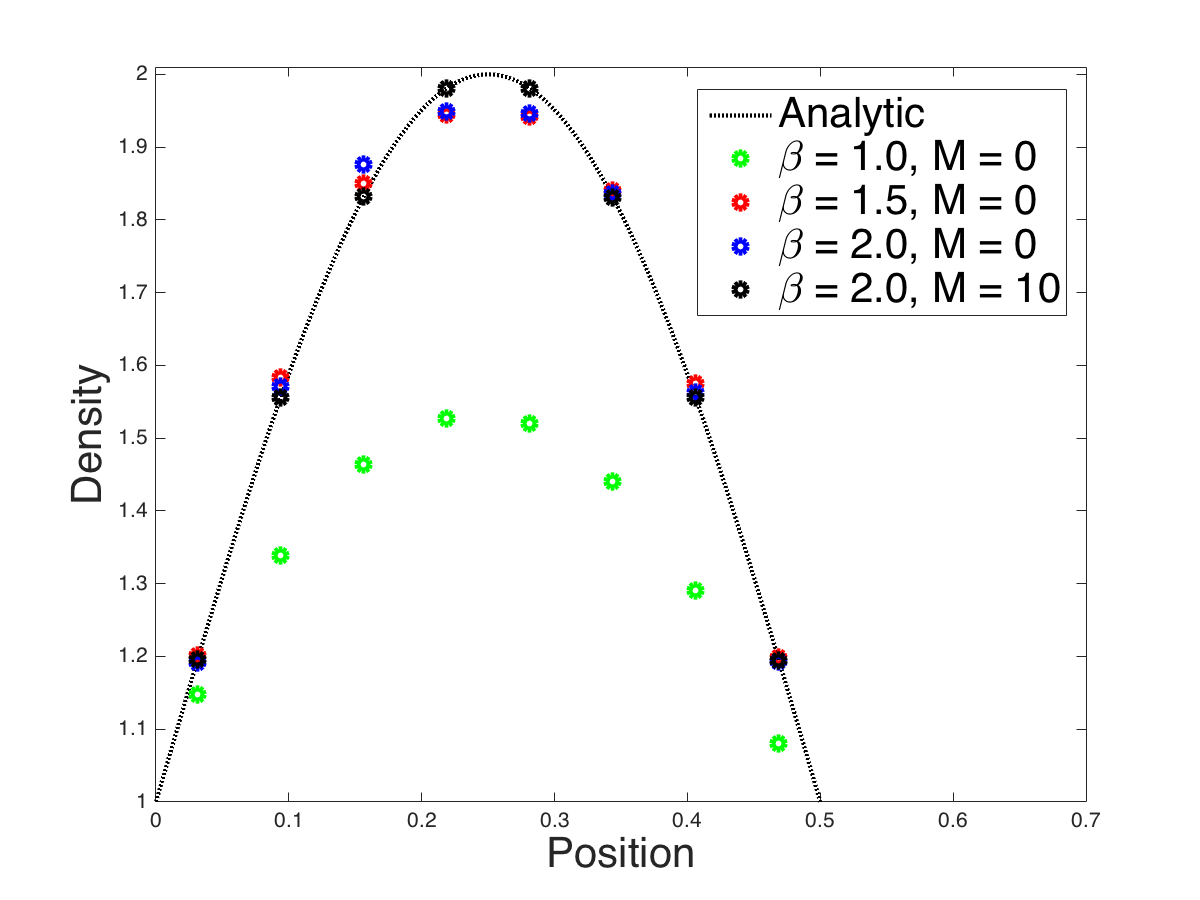
\includegraphics[scale=0.78]{./Figures/StreamingSineWave1D}
  \end{center}
  \caption{Particle density versus position after ten grid crossings ($t=10$) for the streaming sine wave problem computed with the DG(2)+RK3 scheme using 16 elements.  
  We compare results obtained using various limiter parameters (open circles; see text for details) with the analytic solution (dotted line).  
  Results obtained using the discontinuity detector (D) is denoted with black open circles.}
  \label{fig:streamingSineWave}
\end{figure}

\begin{table}
  \begin{center}
  \caption{$L^{\infty}$ error and convergence rates for the streaming sine wave problem.}
  \label{tab:streamingSineWave}
  \begin{tabular}{ccccccccc}
    & \multicolumn{4}{c}{SSP-RK2} & \multicolumn{4}{c}{SSP-RK3} \\
    \cmidrule(r){2-5} \cmidrule(r){6-9}
    $N$ & DG(1) & Rate & DG(2) & Rate & DG(2) & Rate & DG(3) & Rate \\
    \midrule \midrule
    8     & $3.493\times10^{-1}$ & ---  & $9.082\times10^{-3}$ & ---  & $3.310\times10^{-3}$ & ---  & $1.151\times10^{-4}$  & --- \\
    16   & $5.793\times10^{-2}$ &2.59& $2.310\times10^{-3}$ &1.98& $2.652\times10^{-4}$ &3.64& $8.929\times10^{-6}$ &3.69 \\
    32   & $8.423\times10^{-3}$ &2.78& $6.117\times10^{-4}$ &1.92& $3.170\times10^{-5}$ &3.06& $7.911\times10^{-7}$ &3.50 \\
    64   & $1.314\times10^{-3}$ &2.68& $1.574\times10^{-4}$ &1.96& $3.949\times10^{-6}$ &3.00& $7.843\times10^{-8}$ &3.33 \\
    128 & $2.336\times10^{-4}$ &2.49& $3.987\times10^{-5}$ &1.98& $4.934\times10^{-7}$ &3.00& $8.524\times10^{-9}$ &3.20 \\
    256 & $4.736\times10^{-5}$ &2.30& $1.003\times10^{-5}$ &1.99& $6.162\times10^{-8}$ &3.00& $9.997\times10^{-10}$ &3.09 \\
    \midrule \midrule
  \end{tabular}
  \end{center}
\end{table}

\subsection{Spherical Wave}

This problem in spherical symmetry is taken from \citet{pons_etal_2000}, and consists of a gaussian-shaped wave propagating in the radial direction.  
The computational domain is given by $D=\{r:r\in[0.2,10.2]\}$.  
The analytical solution is given by
\begin{equation}
  \cJ(r,t)=\cH_{r}(r,t)
  =\exp\big[-\big(r-t\big)^{2}\big]/r^{2}.  
\end{equation}
We let the boundary conditions be given by the analytical solution, and integrate in time from $t=0$ to $t=7$.  

Snapshots of the solution ($\cJ$ versus $r$), obtained with the DG(2)+RK3 scheme, are shown in Figure~\ref{fig:sphericalWave} for $t=\{2.5,3.5,5.0,7.0\}$ (open circles).  
For comparison, the analytical solution is plotted with dotted lines.  
There is good agreement between the numerical and analytical solutions.  
In Table~\ref{tab:sphericalWave} we list convergence results obtained with the various schemes.  
High-order accuracy is achieved with the DG(2)+RK3 and DG(3)+RK3 schemes.  

\begin{figure}
  \begin{center}
    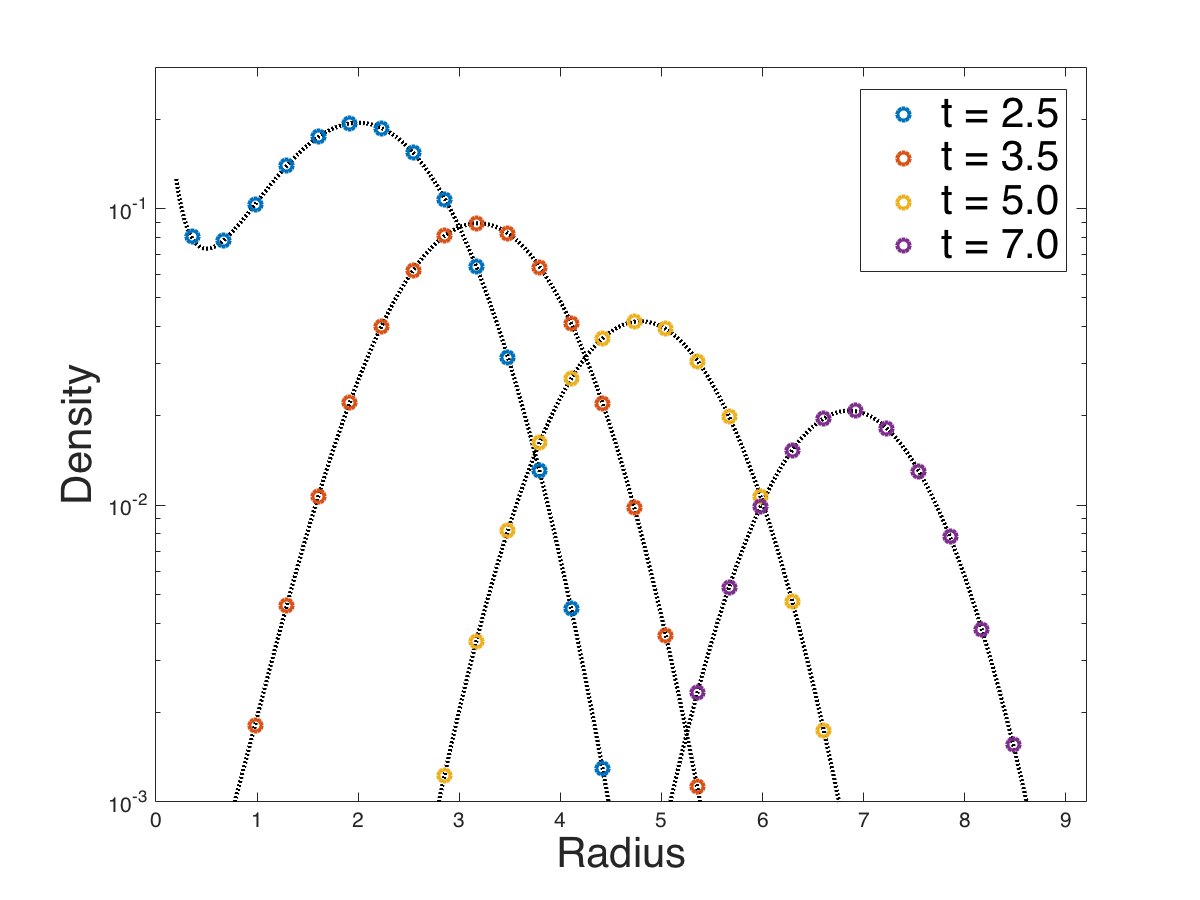
\includegraphics[scale=0.78]{./Figures/GaussianSphericalWave1D}
  \end{center}
  \caption{Energy density versus radius at various times for the spherical wave problem computed with the DG(2)+RK3 scheme using 32 elements.  The numerical solution (open circles) is compared to the analytical solution (dotted lines).  }
  \label{fig:sphericalWave}
\end{figure}

\begin{table}
  \begin{center}
  \caption{$L^{\infty}$ error and convergence rates for the spherical wave problem.}
  \label{tab:sphericalWave}
  \begin{tabular}{ccccccccc}
    & \multicolumn{4}{c}{SSP-RK2} & \multicolumn{4}{c}{SSP-RK3} \\
    \cmidrule(r){2-5} \cmidrule(r){6-9}
    $N$ & DG(1) & Rate & DG(2) & Rate & DG(2) & Rate & DG(3) & Rate \\
    \midrule \midrule
    32   & $4.648\times10^{-4}$ & ---  & $5.540\times10^{-5}$ & ---   & $4.803\times10^{-5}$ & ---  & $1.707\times10^{-5}$ & --- \\
    64   & $9.506\times10^{-5}$ &2.29& $1.088\times10^{-5}$ &2.35& $1.373\times10^{-5}$ &1.81& $7.812\times10^{-7}$ &4.45 \\
    128 & $1.996\times10^{-5}$ &2.25& $1.502\times10^{-6}$ &2.86& $1.836\times10^{-6}$ &2.90& $1.150\times10^{-7}$ &2.76 \\
    256 & $5.783\times10^{-6}$ &1.79& $2.529\times10^{-7}$ &2.57& $1.895\times10^{-7}$ &3.28& $6.268\times10^{-9}$ &4.20 \\
    \midrule \midrule
  \end{tabular}
  \end{center}
\end{table}

\subsection{Line Source}

\subsection{Riemann Problem}

To test the ability of the DG method to capture discontinuities without spurious oscillations, we solve the Riemann problem presented by \citet{OHF2012}.  
This problem is also challenging because the condition $\cJ-|\bcH|>0$ can be violated.  
To compare with the results of \citet{OHF2012}, we use the Eddington factor due to Levermore \citep{levermore_1984}
\begin{equation}
  \psi(h)=\f{1}{3}\big(\,5-2\,\sqrt{4-3\,h^{2}}\,\big).  
  \label{eq:eddingtonFactorLevermore}
\end{equation}
The computational domain extends from $x=-0.05$ to $x=0.1$, and a discontinuity is located at $x_{\mbox{\tiny d}}=0.0$.  
The initial condition is given by
\begin{equation}
  \bcM(x,t=0)=
  \left\{
  \begin{array}{l}
  \bcM_{\mbox{\tiny L}}=\big(1,0.9999,0,0\big)^{T} \quad\text{if}\quad x\le x_{\mbox{\tiny d}} \\
  \bcM_{\mbox{\tiny R}}=\big(0.5,0,0,0\big)^{T} \quad\text{otherwise}.
  \end{array}
  \right.
  \label{eq:riemannProblem}
\end{equation}
Results for $t=0.1$ are shown in Figure~\ref{fig:riemannProblem}.  
In the left panel we plot the number density and flux, obtained with the third-order method (DG(2)+RK3).  
The discontinuities remain sharp, and oscillations around the discontinuities are controlled (in part due to limiting of characteristic variables; cf. Section~\ref{sec:slopeLimiters}).  
In the right panel we plot the number density for three computations: limiting triggered everywhere (blue), no slope limiting (positivity limiting only; red), and limiting triggered by the discontinuity detector (black).  
In the plot we have zoomed in on the discontinuity around $x=0.075$.  
Without limiting, significant oscillations are present in the solution.  
With the slope limiter, the oscillations are essentially removed, while using the discontinuity detector to trigger limiting maintains a sharper discontinuity than when limiting is permitted everywhere.  

\begin{figure}
  \begin{center}
    \begin{tabular}{cc}
      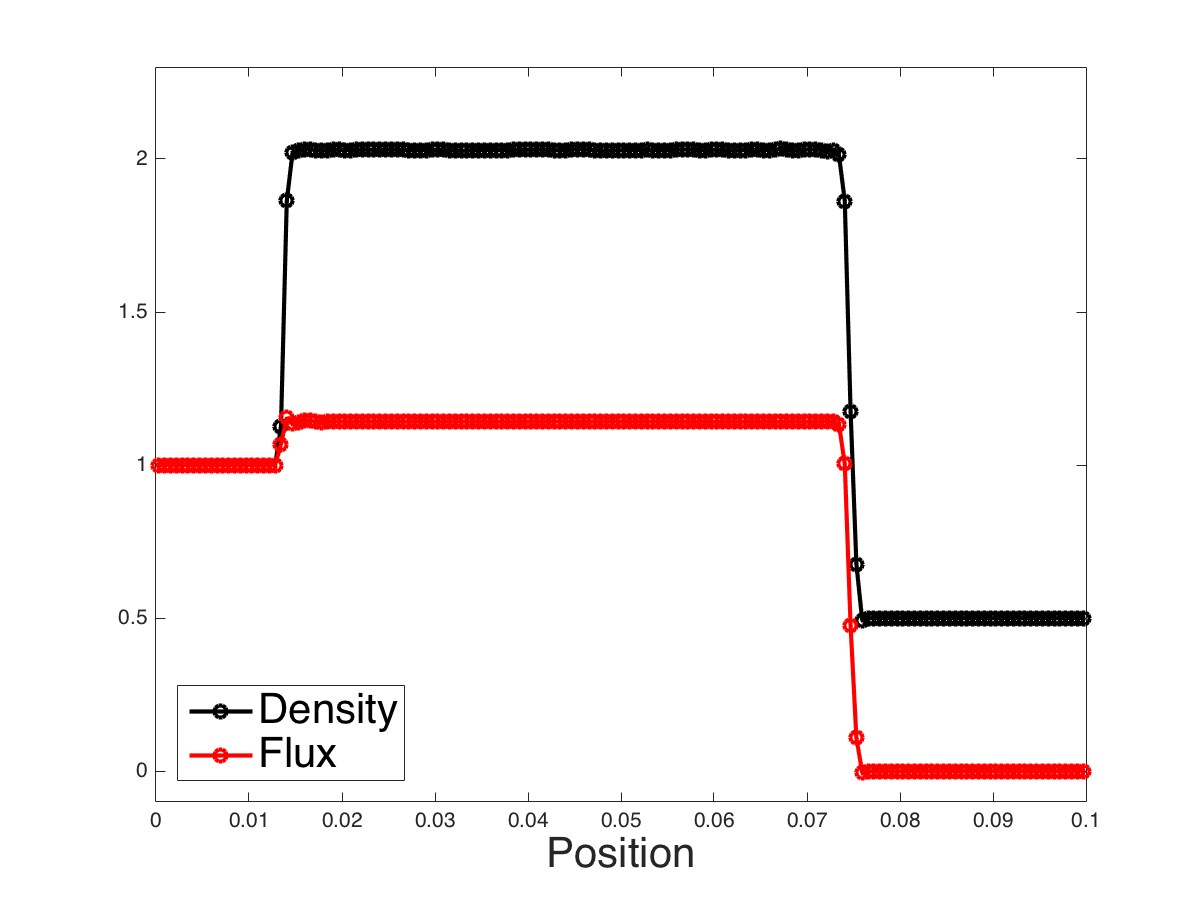
\includegraphics[scale=0.4]{./Figures/RiemannProblem1D} &
      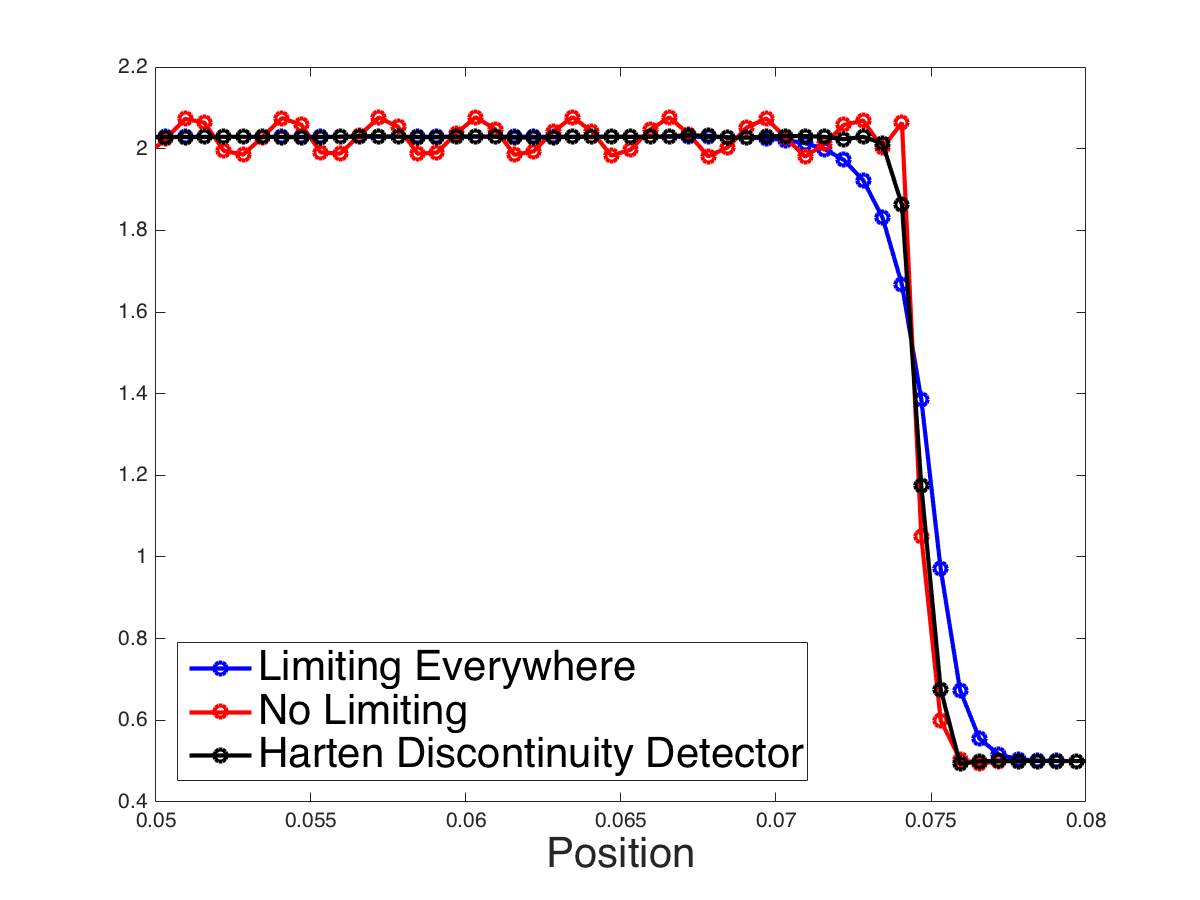
\includegraphics[scale=0.4]{./Figures/RiemannProblem1D_Limiters}
    \end{tabular}
  \end{center}
  \caption{Results from the one-dimensional Riemann problem in Eq.~\eqref{eq:riemannProblem}, obtained with the DG(2)+RK3 method using $240$ elements, the HLL Riemann solver, and the Eddington factor in Eq.~\eqref{eq:eddingtonFactorLevermore}.  
  The number density $\cJ$ (black) and the number flux density $\cH_{1}$ (red) are plotted for $t=0.1$.}
  \label{fig:riemannProblem}
\end{figure}

\subsection{Spherical Diffusion}

Next, we consider a diffusion problem in spherical symmetry, which involves a constant scattering opacity $\sigma$.  
This problem is adapted from \citet{abdikamalov_etal_2012} \citep[see also][]{pons_etal_2000,sumiyoshiYamada_2012}.  
For sufficiently high scattering opacity, the moment equations limit to a diffusion equation for the radiation number density.  
With a Gaussian initial distribution for the energy density $\cJ_{0}(x)=\exp(-3\,\sigma\,r^{2}/(4\,t_{0}))$, the analytical solution to the limiting diffusion equation is given by
\begin{equation}
  \cJ(r,t)=\Big(\f{t_{0}}{t_{0}+t}\Big)^{3/2}\,\exp\Big\{\,-\f{3\,\sigma\,r^{2}}{4\,(t_{0}+t)}\,\Big\},
\end{equation}
while the number flux is obtained from $\cH_{r}=-\pd{\cJ}{r}/(3\,\sigma)$.  

We present two versions of this test:  one with $\sigma=10^{-5}$~cm$^{-1}$ (thin test), and one with $\sigma=10^{-1}$~cm$^{-1}$ (thick test).  
In the thin test, the computational domain extends over $r\in[0,100]$~km, $t_{0}=0.3$~ms, and is run until $t=1$~ms.  
In the thick test, the computational domain extends over $r\in[0,50]$~km and $t_{0}=0.3$~s, and is run until $t=1$~s.  
In both tests we use 32 elements and the DG(2)+SIRK2 scheme.  
With the mean-free path defined as $\lambda=1/\sigma$, the ratio of the mean-free path to the cell width $\Delta r$ is $0.32$ in the thin test, and $6.4\times10^{-5}$ in the thick test.  

Results are plotted in Figure~\ref{fig:diffusionProblem}.  
There is good agreement between the numerical and analytical solutions, for both the thin and thick cases.  

\begin{figure}
  \begin{center}
    \begin{tabular}{cc}
      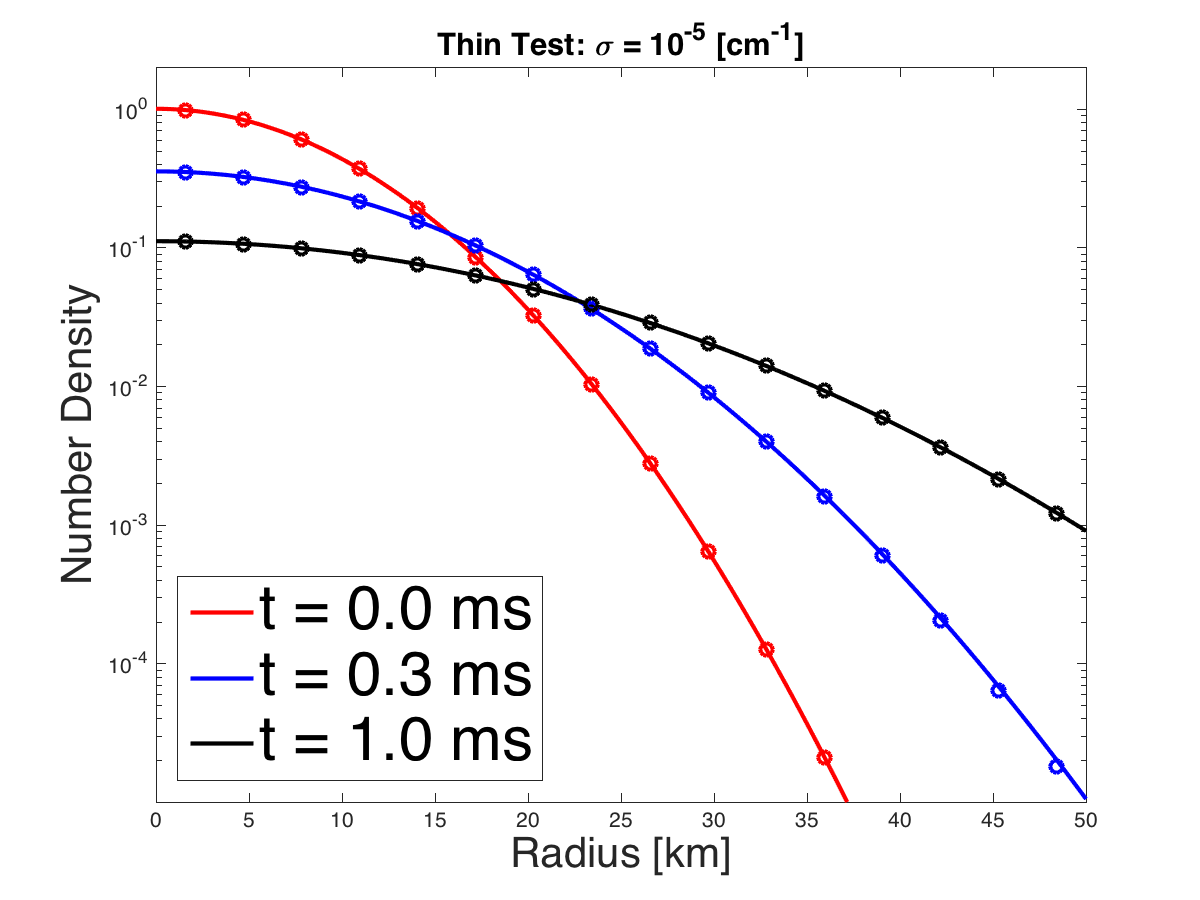
\includegraphics[scale=0.38]{./Figures/GaussianSphericalDiffusion_Kappa_1e-5_Density} &
      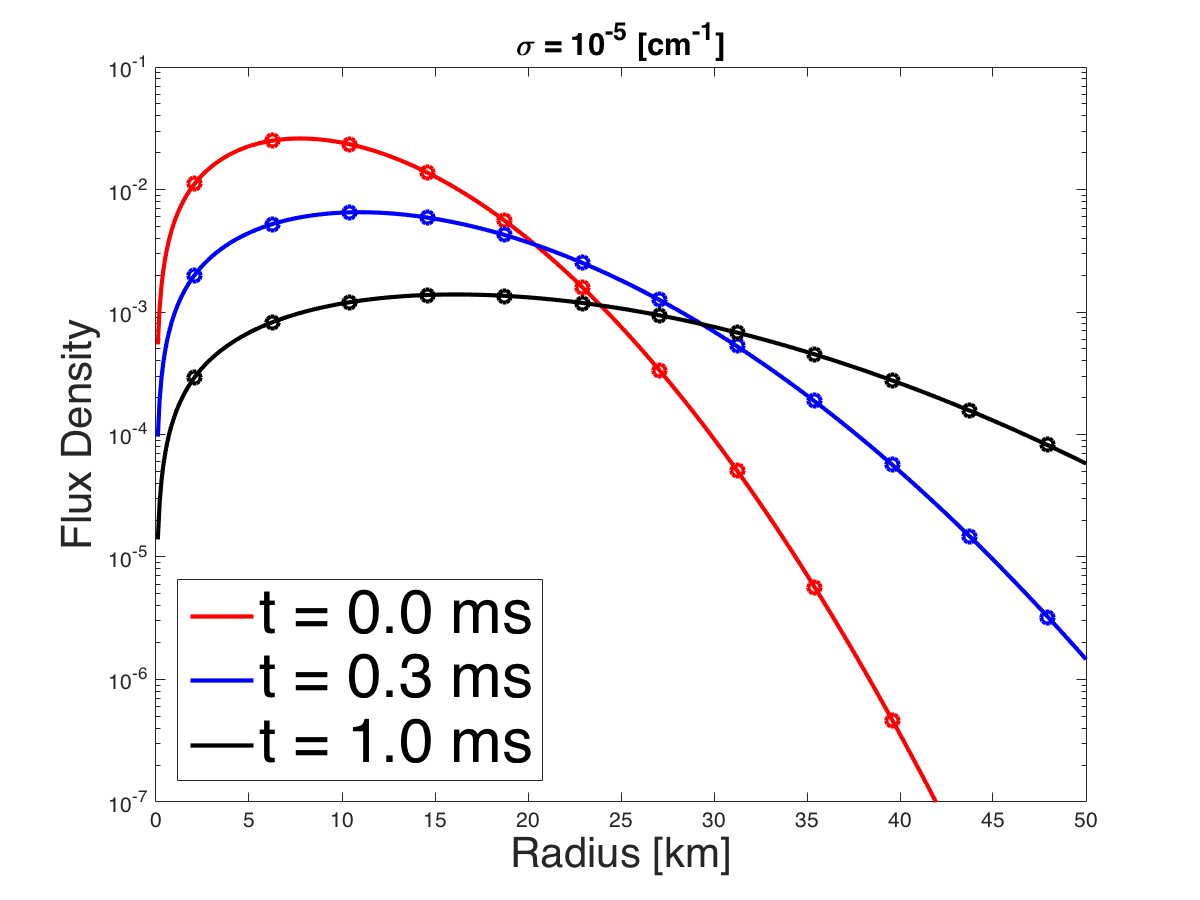
\includegraphics[scale=0.38]{./Figures/GaussianSphericalDiffusion_Kappa_1e-5_Flux} \\
      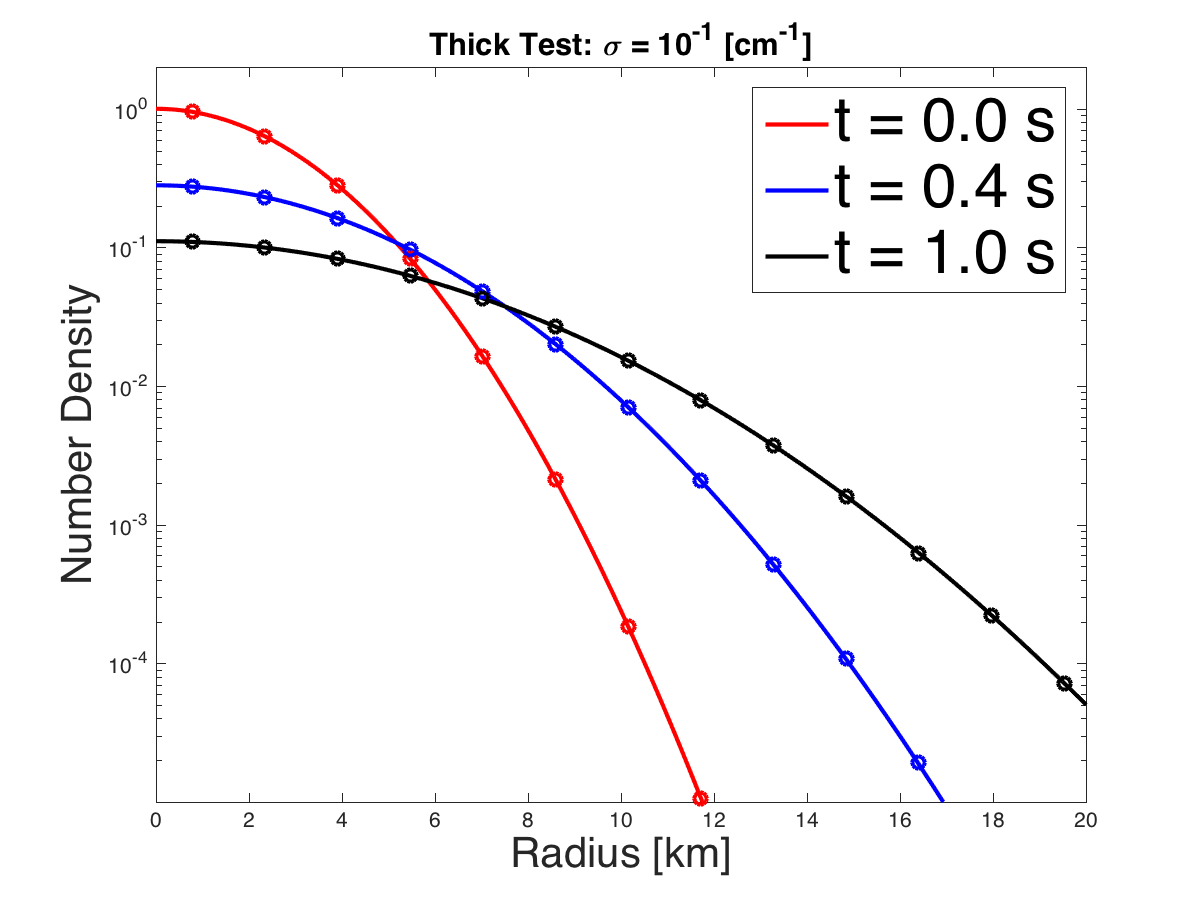
\includegraphics[scale=0.38]{./Figures/GaussianSphericalDiffusion_Kappa_1e-1_Density} &
      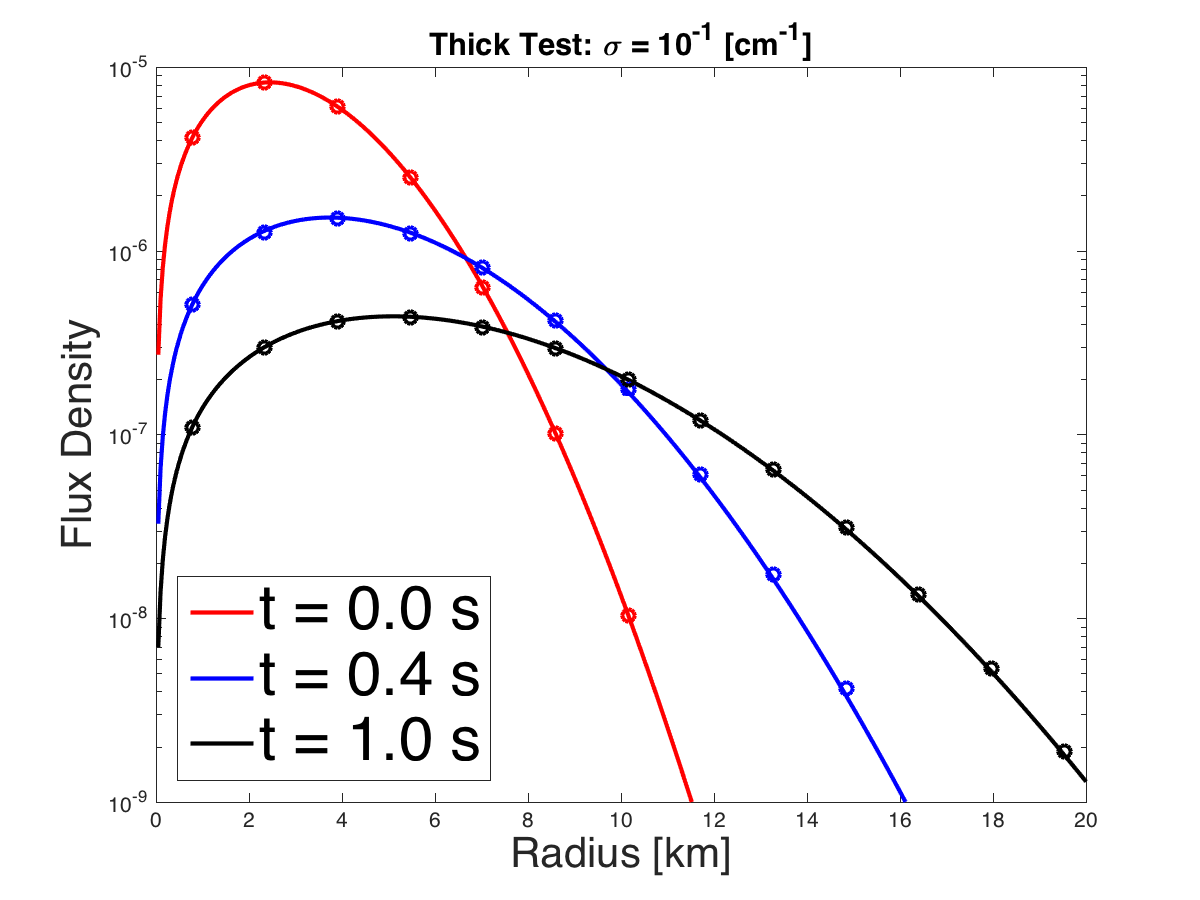
\includegraphics[scale=0.38]{./Figures/GaussianSphericalDiffusion_Kappa_1e-1_Flux}
    \end{tabular}
  \end{center}
  \caption{Results from the one-dimensional diffusion problem in spherical symmetry, obtained with the DG(2)+SIRK2 method using $32$ elements.  
  The number density $\cJ$ (left panel) and the number flux density $\cH_{r}$ (right panel) are plotted.  
  In the upper panels $\sigma=10^{-5}$~cm$^{-1}$, with results plotted for $t=0,0.3,1.0$~ms (red, blue, and black curves, respectively).  
  In the lower panels $\sigma=10^{-1}$~cm$^{-1}$, with results plotted for $t=0,0.4,1.0$~s (red, blue, and black curves, respectively).  
  Solid lines represent the analytical solution while open circles represent the element center value of the numerical solution.}
  \label{fig:diffusionProblem}
\end{figure}

\subsection{Homogeneous Sphere}

The homogeneous sphere test \citep[cf.][]{smit_etal_1997} considers of a sphere with radius $R$.  
Inside the sphere ($r<R$), the absorption opacity and equilibrium distribution function are set to constant values $\chi=\chi_{0}$ and $f_{0}=1$, respectively.  
Outside the sphere, the absorption opacity is zero.  
The steady state solution, obtained by solving the transport equation in spherical symetry, is given by
\begin{equation}
  f_{\mbox{\tiny A}}(r,\mu)=f_{0}\,\big(1-e^{-\chi_{0}\,s(r,\mu)}\big),
  \label{distributionHomogeneousSphere}
\end{equation}
where
\begin{equation}
  s(r,\mu)
  =\left\{
  \begin{array}{lll}
    r\,\mu+R\,g(r,\mu) & \mbox{if}\quad r<R, & \mu\in[-1,+1], \\
    2\,R\,g(r,\mu) & \mbox{if}\quad r \ge R, & \mu\in[(1-(R/r)^{2})^{1/2},+1], \\
    0 & \mbox{otherwise},
  \end{array}
  \right.
\end{equation}
and $g(r,\mu)=[1-(r/R)^{2}(1-\mu^{2})]^{1/2}$.  

Similar to \citet{oConnor_2015}, we solve two versions of this test.  
One where the absorption opacity is set to $\chi_{0}=10^{-4}$~cm$^{-1}$ (thick; similar to the electron capture opacity encountered in the center of a collapsed stellar core), and one where the absorption opacity is set to $\chi_{0}=10^{-6}$~cm$^{-1}$ (thin).  
Both simulations are run with a computational domain with $r\in[0,500]$~km using 100 uniform elements $\Delta r=5$~km.  
Thus, in the thick case, the Knudsen number is small, $\mbox{Kn}=(\chi_{0}\,\Delta r)^{-1}=0.02$, while it exceeds unity in the thin case, $\mbox{Kn}=2$.  
The radius of the sphere is set to $R=100$~km.  

Results are plotted in Figure~\ref{fig:homogeneousSphere1D}.  

\begin{figure}
  \begin{center}
    \begin{tabular}{cc}
      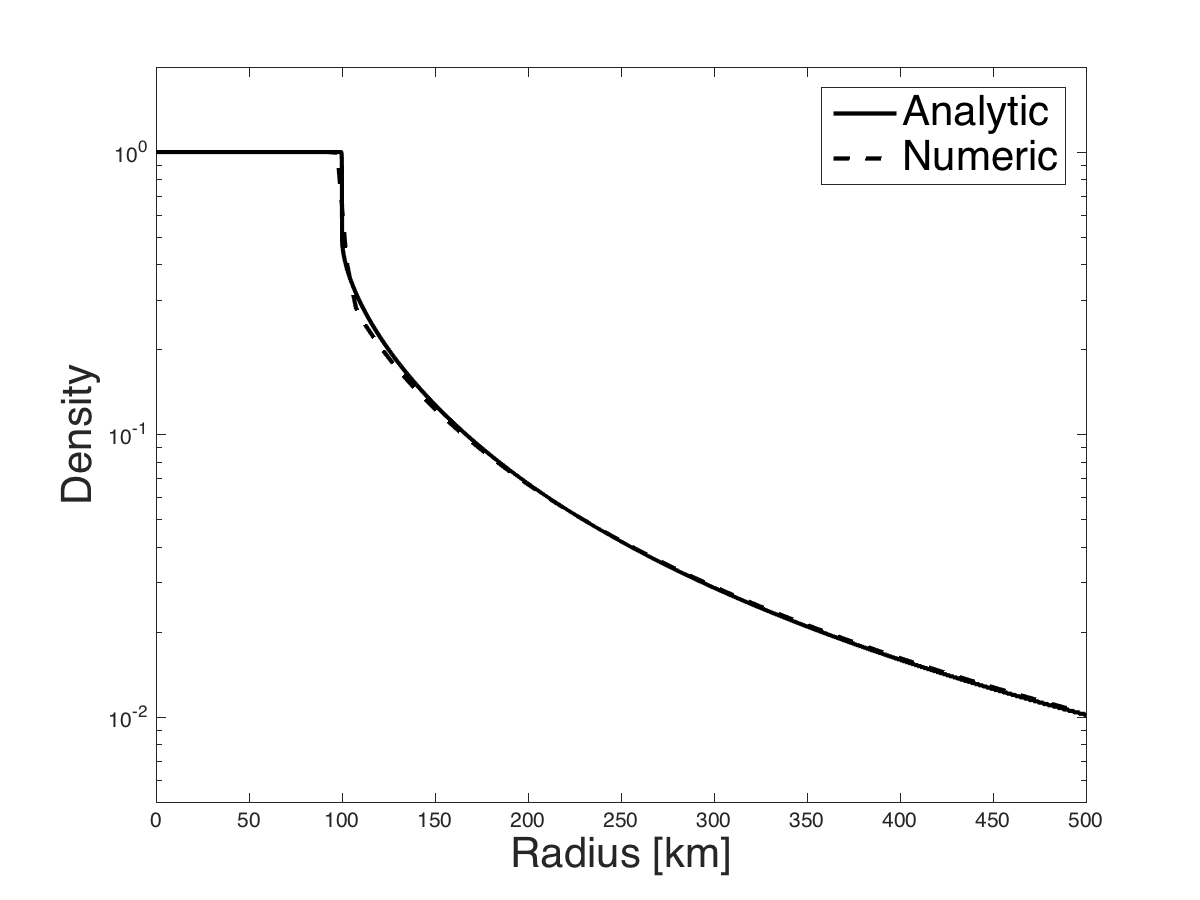
\includegraphics[scale=0.4]{./Figures/HomogeneousSphere1D_Chi_1e-4_Density} &
      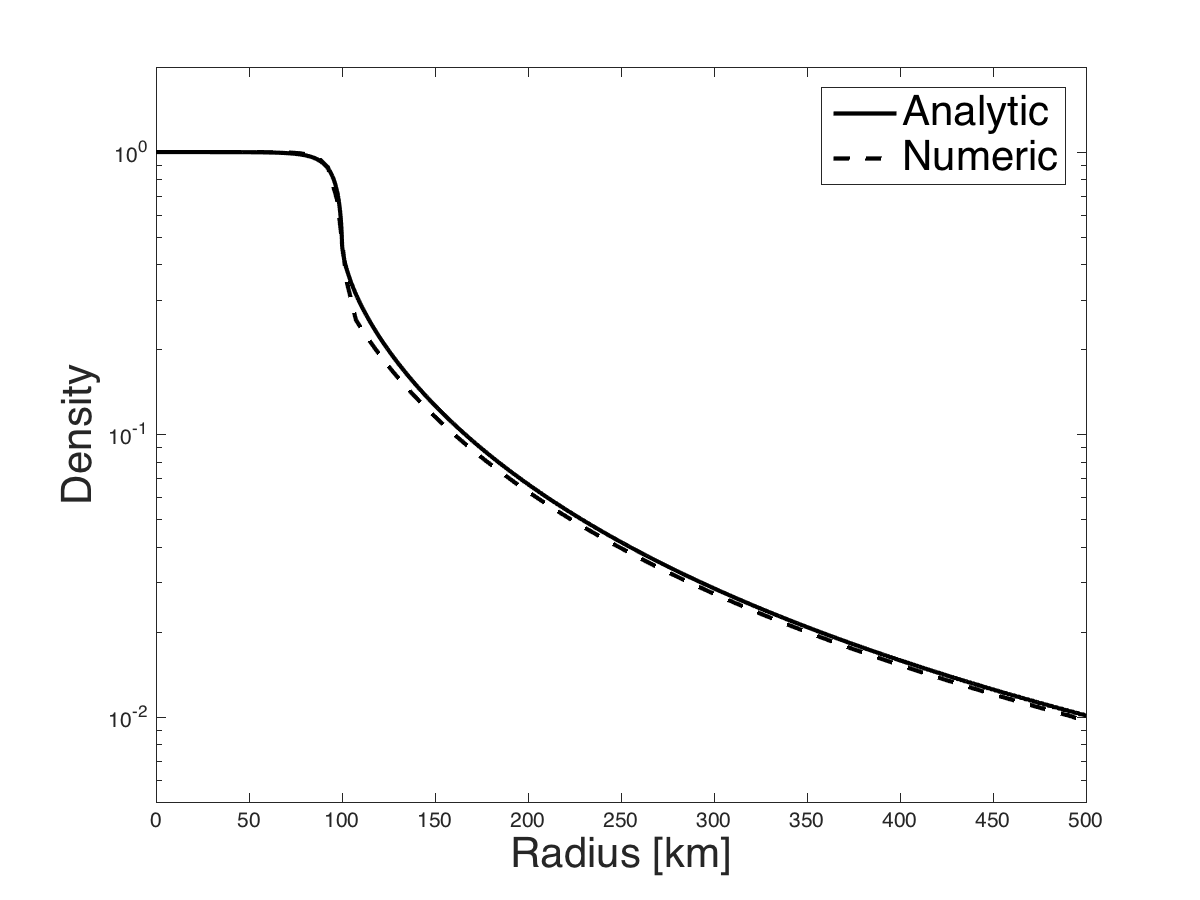
\includegraphics[scale=0.4]{./Figures/HomogeneousSphere1D_Chi_1e-6_Density} \\
      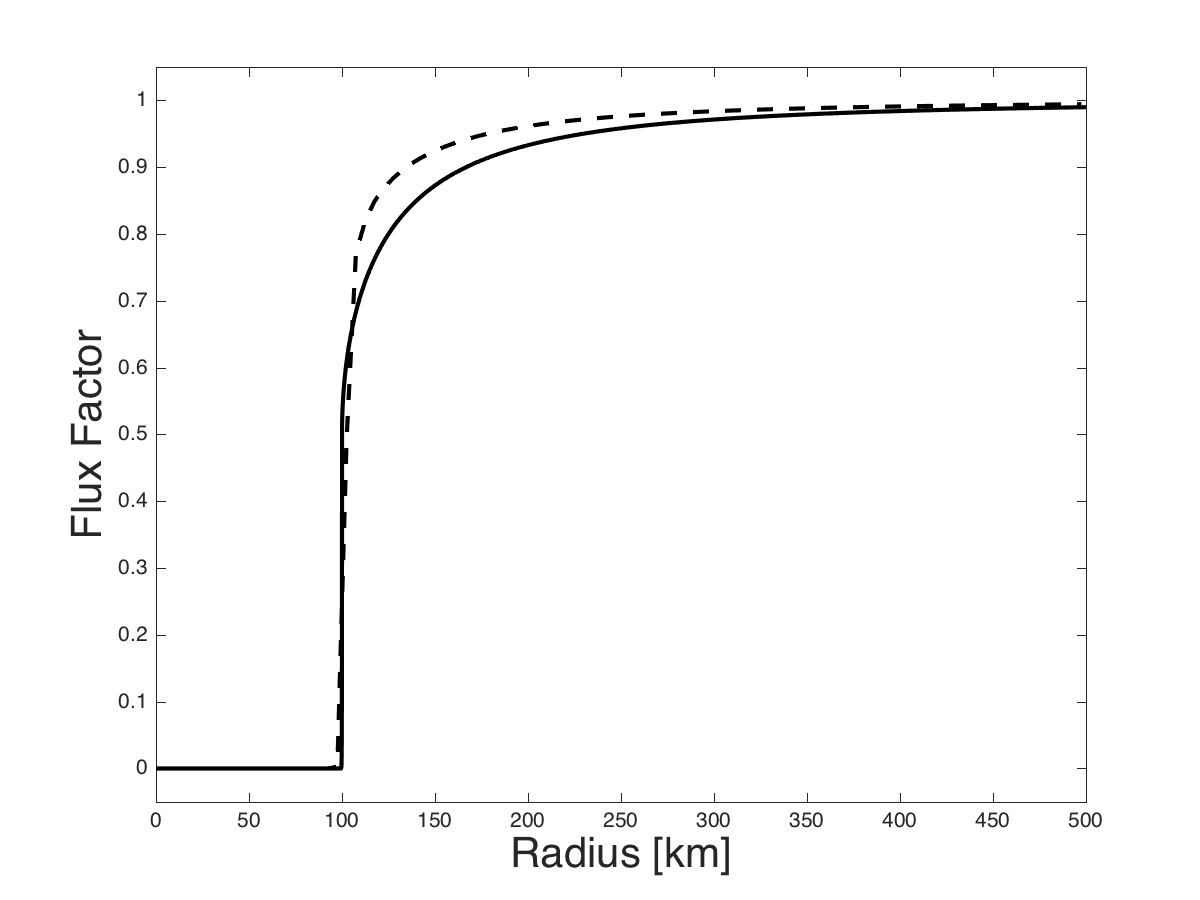
\includegraphics[scale=0.4]{./Figures/HomogeneousSphere1D_Chi_1e-4_FluxFactor} &
      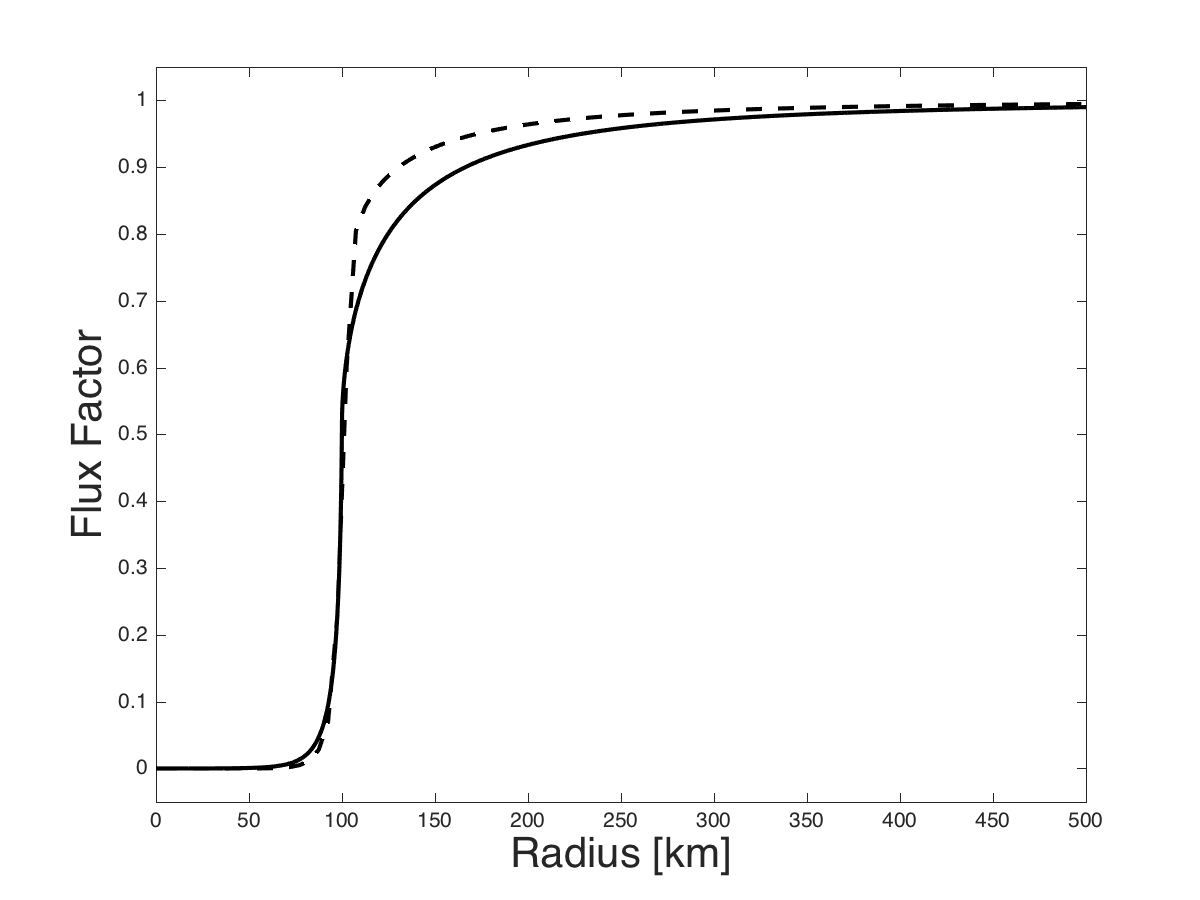
\includegraphics[scale=0.4]{./Figures/HomogeneousSphere1D_Chi_1e-6_FluxFactor} \\
      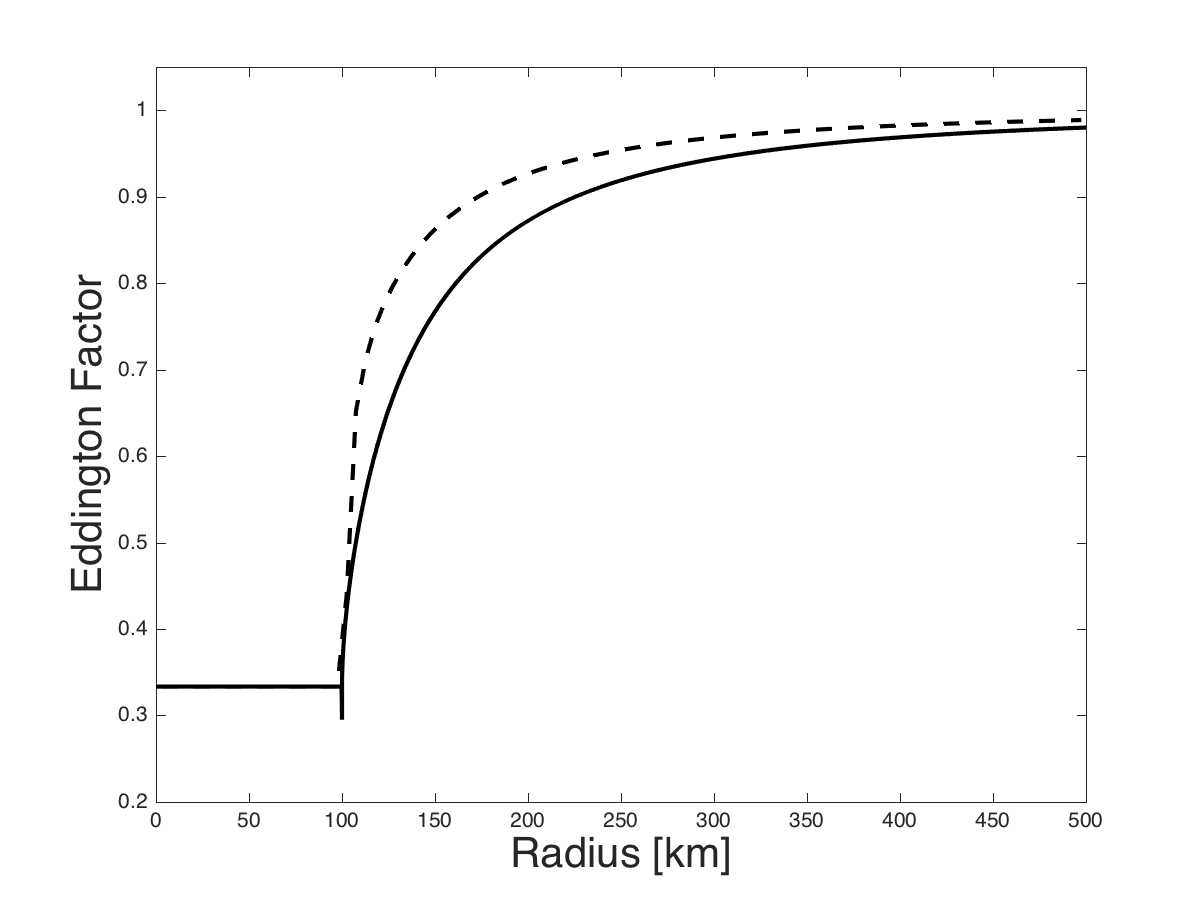
\includegraphics[scale=0.4]{./Figures/HomogeneousSphere1D_Chi_1e-4_EddingtonFactor} &
      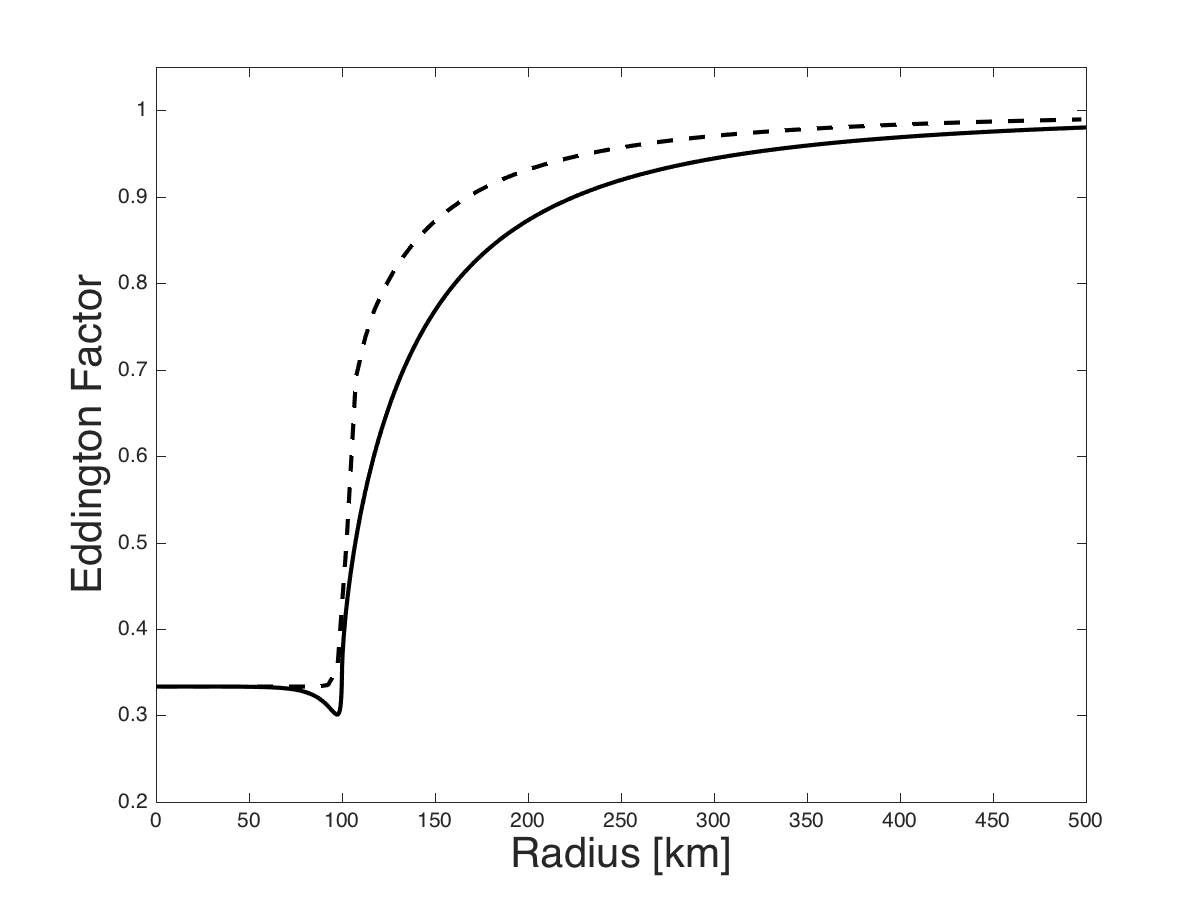
\includegraphics[scale=0.4]{./Figures/HomogeneousSphere1D_Chi_1e-6_EddingtonFactor}
    \end{tabular}
  \end{center}
  \caption{Results from solving the Homogeneous sphere problem with the DG(2)+SIRK2 method using $100$ elements.  
  In the left panels, the absorption opacity is set to $\chi_{0}=10^{-4}$~cm$^{-1}$, while in the right panels it is set to $\chi_{0}=10^{-6}$~cm$^{-1}$.  
  The numerical results (dashed lines) are compared to the analytical solution (solid lines).}
  \label{fig:homogeneousSphere1D}
\end{figure}

\subsection{Milne's Problem}

\section{Mini-app: Transport Problems with Tabulated Neutrino Opacities}

For the tests in this section we employ the tabulated opacities described in Section~\ref{sec:opacities}.  
We present two tests from the previous section (the homogeneous sphere and spherical diffusion problems), where the background is kept fixed.  
Then we present a relaxation problem involving neutrino-electron scattering (NES) with a homogeneous background.  
Finally, we present a deleptonization problem where the background density mimics that of a collapsed stellar core.  
The first deleptonization problem (Em/Ab) involves emission and absorption only, while the second deleptonization problem (Full) involves the full set of opacities described in Section~\ref{sec:opacities}.  

When coupling neutrinos to the background fluid, the gain/loss terms involve integrals of the right-hand sides in Eqs.~\eqref{eq:momentEquationEnergy} and \eqref{eq:momentEquationMomentum} over energy space.  
To simulate multi-group neutrino transport and compute the lepton and energy exchange with the fluid, the infinite energy domain $\bbR^{+}$ is replaced with a finite domain $D^{\epsilonNu}=\{\epsilonNu~|~\epsilonNu\in[0,\epsilonNu_{\mbox{\tiny max}}]\}$.  
The domain $D^{\epsilonNu}$ is then split up into $N_{\epsilonNu}$ energy bins $K_{i}^{\epsilonNu}=\{\epsilonNu~|~\epsilonNu\in[\epsilonNu_{i-1/2},\epsilonNu_{i+1/2}]\}$, where the width of the $i$th bin is $|K_{i}^{\epsilonNu}|=(\epsilonNu_{i+1/2}-\epsilonNu_{i-1/2})$.  
Within each bin, we employ a polynomial representation of the radiation fields and solve for nodal values collocated in Gaussian quadrature points.  
The number of quadrature points $N$ then increases with the degree $k$ of the polynomial representation ($N=k+1$).  
Integrals of radiation quantities over energy space are then evaluated as
\begin{equation}
  \int_{\bbR^{+}}g(\epsilonNu)\,d\epsilonNu
  \approx\int_{D^{\epsilonNu}}g(\epsilonNu)\,d\epsilonNu
  =\sum_{i=1}^{N^{\epsilonNu}}\int_{K_{i}^{\epsilonNu}}g(\epsilonNu)\,d\epsilonNu
  \approx\sum_{i=1}^{N^{\epsilonNu}}|K_{i}^{\epsilonNu}|\sum_{q=1}^{N}w_{q}\,g_{q}=\sum_{j=1}^{M^{\epsilonNu}} W_{j}\,g_{j}=\vect{W}\cdot\vect{g},
\end{equation}
where $w_{q}$ are Gaussian quadrature weights (normalized such that $\sum_{q=1}^{N}w_{q}=1$) and $M^{\epsilonNu}=N^{\epsilonNu}\times N$.  
In constructing the vectors $\vect{W},\vect{g}\in\bbR^{M^{\epsilonNu}}$, their elements are sorted with energy monotonically increasing with $j$; e.g., $\epsilonNu_{j}=\epsilonNu_{i-1/2}+|K_{i}|\times(1/2+\eta_{q}^{\epsilonNu})$ and $W_{j}=|K_{i}^{\epsilonNu}|\,w_{q}$, where $\eta_{q}^{\epsilonNu}$ is the Gaussian quadrature point on the local reference element ($\eta^{\epsilonNu}\in[-1/2,1/2]$), and $j=(i-1)\times N+q$, ($i=1,\ldots,N^{\epsilonNu}$, $q=1,\ldots,N$).  

\subsection{Fluid-Radiation Coupling}

\subsubsection{Emission and Absorption}

Electron capture on nucleons and nuclei results in changes to the electron fraction and internal energy of the fluid given by
\begin{align}
  d_{t}Y_{e}
  &=-\f{m_{\mbox{\tiny B}}}{\rho}\int_{\bbR^{+}}\tilde{\chi}\,\big(\cJ_{0}-\cJ\big)\,dV_{\epsilonNu}, \label{eq:electronFractionEmAb} \\
  d_{t}\epsilon
  &=-\f{1}{\rho}\int_{\bbR^{+}}\tilde{\chi}\,\big(\cJ_{0}-\cJ\big)\,\epsilonNu\,dV_{\epsilonNu}, \label{eq:internalEnergyEmAb}
\end{align}
where $m_{\mbox{\tiny B}}$ is the baryon mass and $\epsilon$ is the specific internal energy.  
In each implicit step in the SIRK2 scheme discussed in Section~\ref{sec:semiImplicitTime} we solve Eqs.~\eqref{eq:electronFractionEmAb}-\eqref{eq:internalEnergyEmAb} coupled to the collision part of the moment equations.  
\begin{align}
  Y_{e}^{n+1}-Y_{e}^{n}
  &=-\f{m_{\mbox{\tiny B}}}{\rho}\sum_{j=1}^{M^{\epsilonNu}}W_{j}^{(2)}\,\gamma_{j}^{n}\,\big(\cJ_{0,j}^{n+1}-\cJ_{j}^{n+1}\big), \label{eq:electronFractionEmAbDiscrete0} \\
  \epsilon^{n+1}-\epsilon^{n}
  &=-\f{1}{\rho}\sum_{j=1}^{M^{\epsilonNu}}W_{j}^{(3)}\,\gamma_{j}^{n}\,\big(\cJ_{0,j}^{n+1}-\cJ_{j}^{n+1}\big), \label{eq:internalEnergyEmAbDiscrete0}
\end{align}
where $W_{j}^{(2,3)}=w_{q}\,\epsilonNu_{i,q}^{2,3}\,\Delta\epsilonNu_{i}$ and $\gamma_{j}^{n}=\dt\,\tilde{\chi}_{j}^{n}$.  
Note that the absorption opacity is defined at the known time level $t^{n}$, which avoids computation of derivatives with respect to temperature and electron fraction.  
The radiation energy density is updated from
\begin{equation}
  \cJ_{j}^{n+1}=\f{\cJ_{j}^{n}+\gamma_{j}^{n}\,\cJ_{0,j}^{n+1}}{1+\gamma_{j}^{n}}, 
  \label{eq:momentEquationEnergyEmAbDiscrete}
\end{equation}
which, when inserted into Eqs.~\eqref{eq:electronFractionEmAbDiscrete0}-\eqref{eq:internalEnergyEmAbDiscrete0}, results in a nonlinear system for the unknowns $Y^{n+1}$ and $\epsilon^{n+1}$
\begin{align}
  Y_{e}^{n+1}-Y_{e}^{n}
  &=-\f{m_{\mbox{\tiny B}}}{\rho}\sum_{j=1}^{M^{\epsilonNu}}W_{j}^{(2)}\,\tilde{\gamma}_{j}^{n}\,\big(\cJ_{0,j}^{n+1}-\cJ_{j}^{n}\big), \label{eq:electronFractionEmAbDiscrete} \\
  \epsilon^{n+1}-\epsilon^{n}
  &=-\f{1}{\rho}\sum_{j=1}^{M^{\epsilonNu}}W_{j}^{(3)}\,\tilde{\gamma}_{j}^{n}\,\big(\cJ_{0,j}^{n+1}-\cJ_{j}^{n}\big), \label{eq:internalEnergyEmAbDiscrete}
\end{align}
where $\tilde{\gamma}_{j}^{n}=\gamma_{j}^{n}/(1+\gamma_{j}^{n})$.  
Since the equilibrium density $\cJ_{0,j}$ is a nonlinear function of $Y_{e}$ and $\epsilon$, Eqs.~\eqref{eq:electronFractionEmAbDiscrete}-\eqref{eq:internalEnergyEmAbDiscrete} are solved using Newton's method.  
Once $Y_{e}^{n+1}$ and $\epsilon^{n+1}$ are obtained, the radiation density is obtained from Eq.~\eqref{eq:momentEquationEnergyEmAbDiscrete}, while the flux is given by
\begin{equation}
  \bcH_{j}^{n+1}=\bcH_{j}^{n}/(1+\gamma_{j}^{n}).  
  \label{eq:momentEquationMomentumEmAbDiscrete}
\end{equation}

\subsubsection{Neutrino-Electron Scattering}

\subsubsection{Full Interaction Set}

\begin{table}
  \caption{Parameters used for problems with tabulated opacities. \label{tab:tabulatedModels}}
  \begin{tabular}{ccccc}
    Model & $\rho$ [g~cm$^{-3}$] & $T$ [MeV] & $Y_{e}$ & $\mu_{\nu}$ [MeV] \\
    \midrule \midrule
    A & $1.0\times10^{14}$ & 21.0  & 0.25 &   90.65 \\
    B & $1.0\times10^{13}$ & 16.0 & 0.14 &     4.80 \\
    C & $1.0\times10^{12}$ &   8.0 & 0.12 & -   0.57 \\
    D & $1.0\times10^{11}$ &   8.0 & 0.15 & - 10.87 \\
    \midrule \midrule
  \end{tabular}
\end{table}

\subsection{Homogeneous Sphere}

\begin{figure}
  \begin{center}
    \begin{tabular}{cc}
      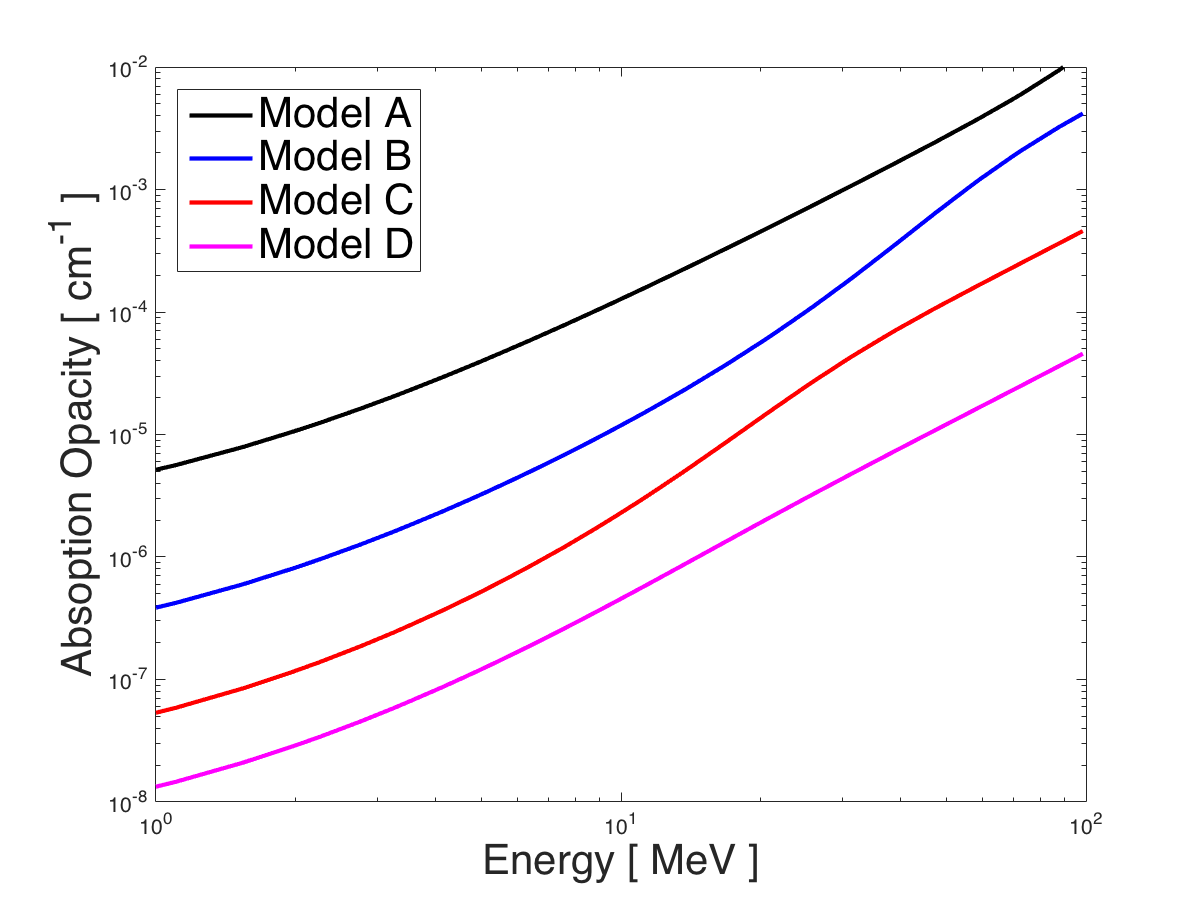
\includegraphics[scale=0.4]{./Figures/HomogeneousSphere_Opacities} &
      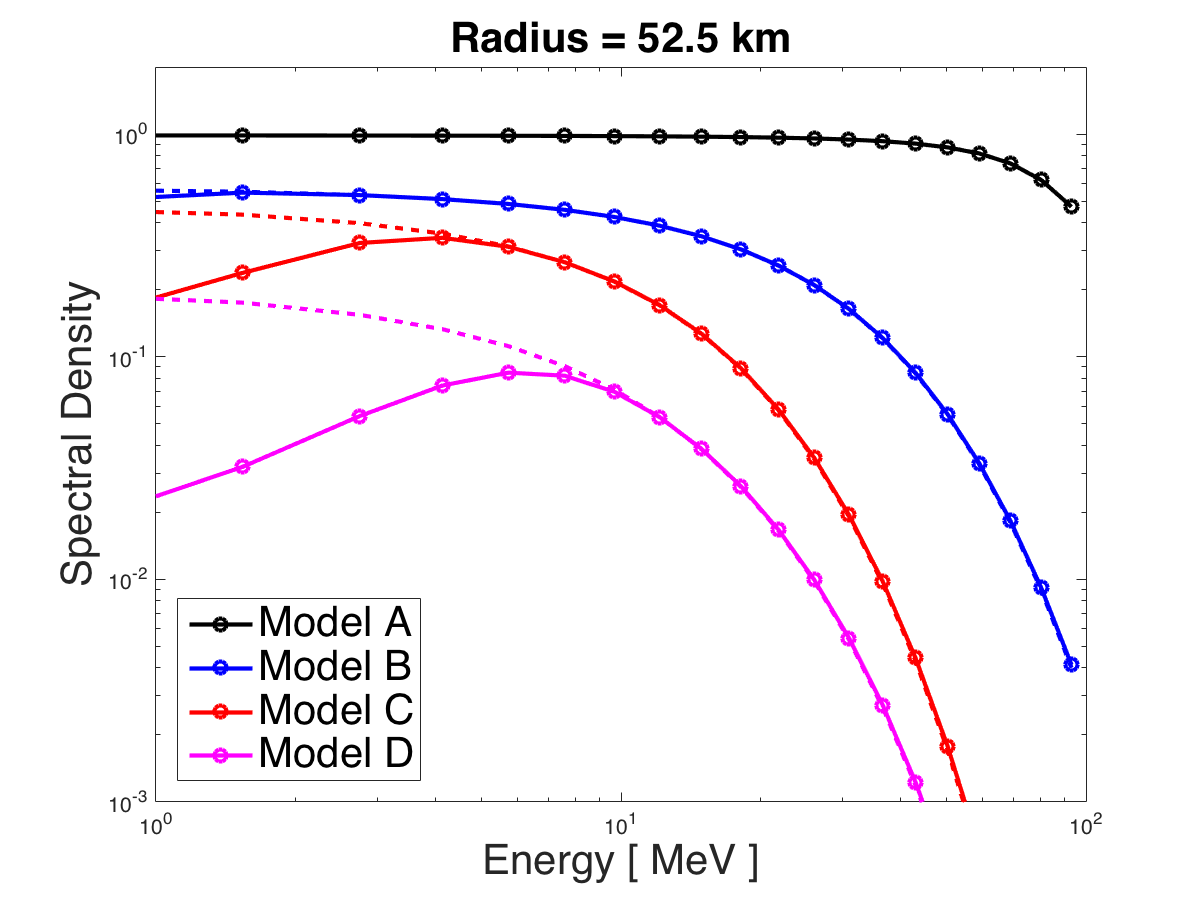
\includegraphics[scale=0.4]{./Figures/HomogeneousSphere_BaseSpectra} \\
      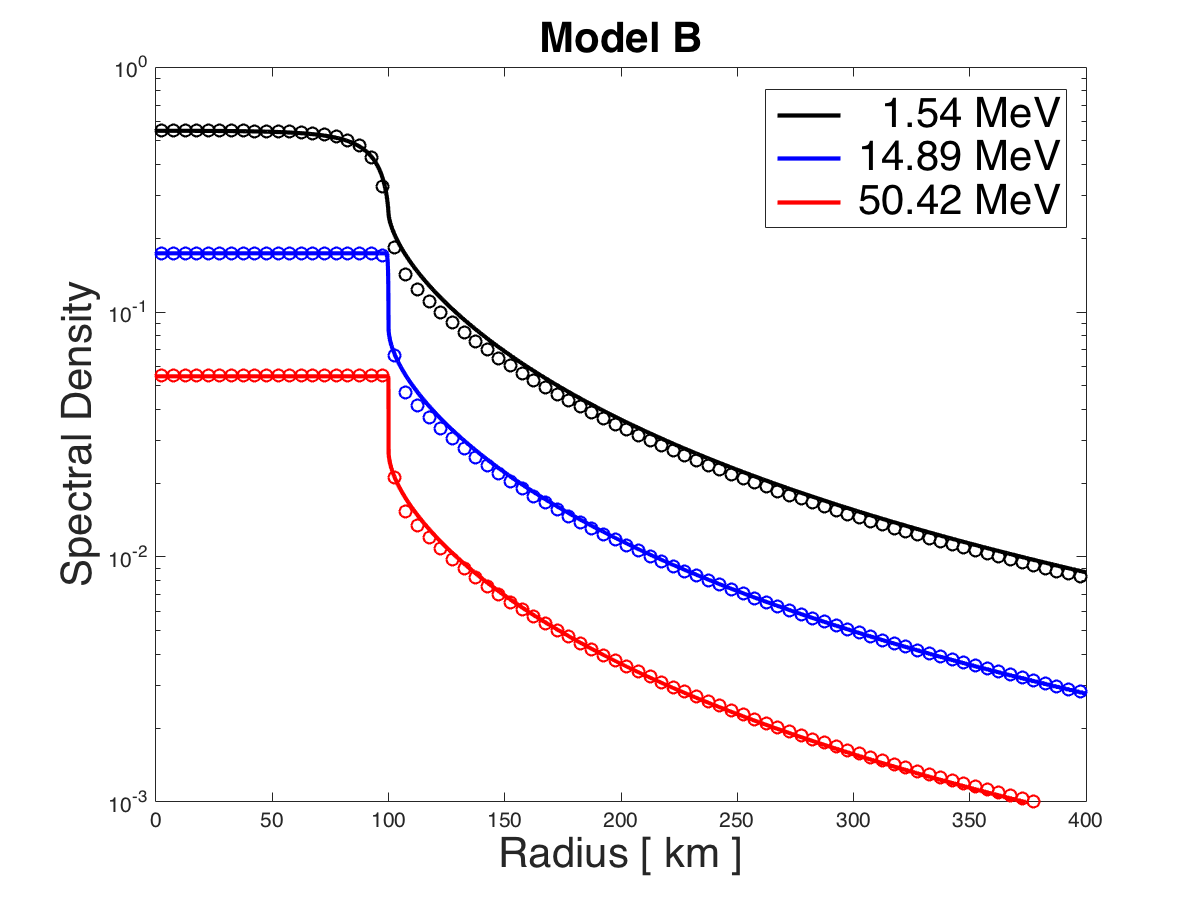
\includegraphics[scale=0.4]{./Figures/HomogeneousSphere_VsRadius_B} &
      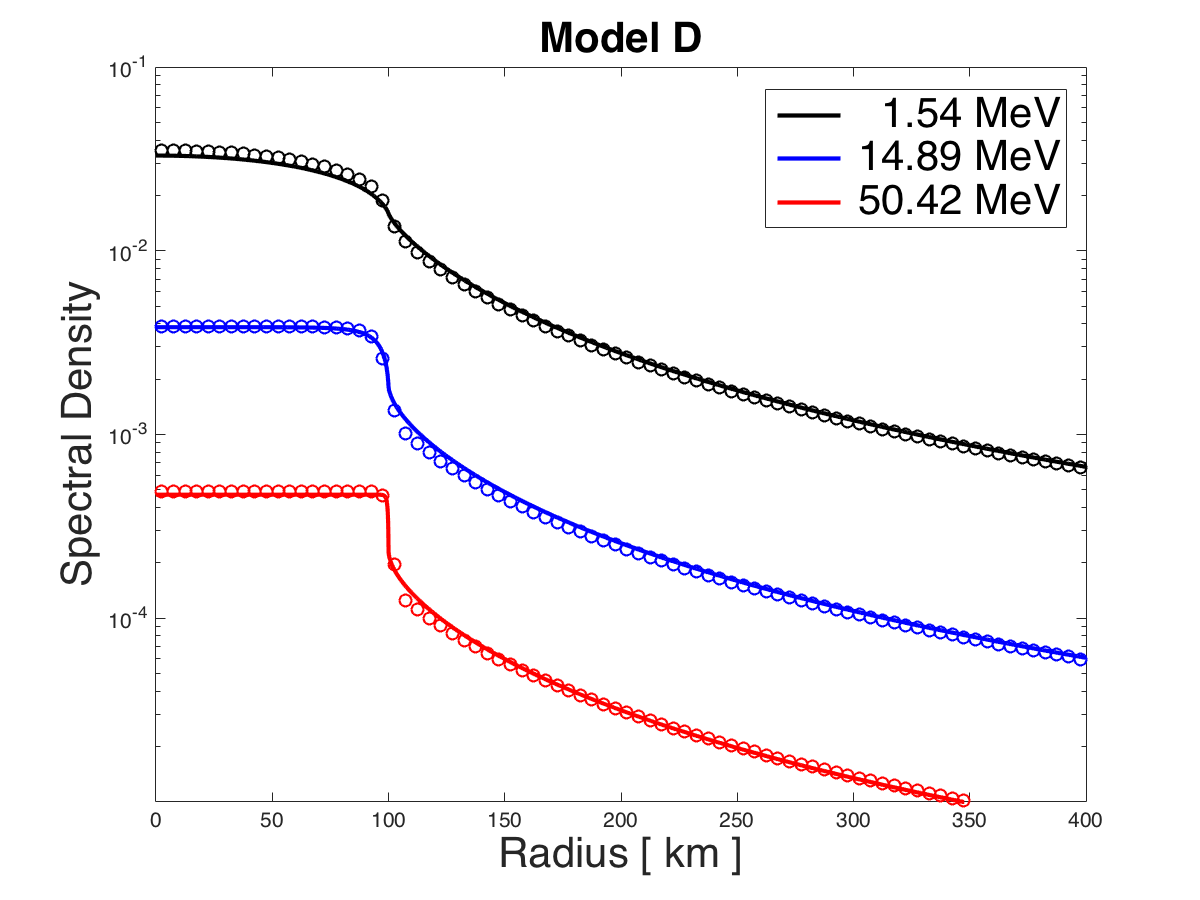
\includegraphics[scale=0.4]{./Figures/HomogeneousSphere_VsRadius_D}
    \end{tabular}
  \end{center}
  \caption{Results from solving the multi-group Homogeneous sphere problem with the DG(1)+SIRK2 method using $100$ elements.
    In the upper left panel we plot the absorption opacity versus energy $\epsilonNu$ using the values for $\rho$, $T$, and $Y_{e}$ listed in Table~\ref{tab:tabulatedModels}. In the upper right panel, we plot the spectral number density versus energy at the end of the computations for a radius of $52.5$~km solid lines.  The corresponding Fermi-Dirac spectrum is also plotted (dashed lines).  }
  \label{fig:homogeneousSphere1D_weaklib}
\end{figure}

\subsection{Diffuse Scattering}

\subsection{Relaxation}

\subsection{Deleptonization}

We conclude with a problem mimicking the deleptonization of a collapsed stellar core.  
To this end, we adopt an analytic density profile
\begin{equation}
  \rho(r)=\big[\,1-\Theta(r)\,\big]\,\rho_{1}(r)+\Theta(r)\,\rho_{2}(r)
  \label{eq:densityProfile}
\end{equation}
where the function $\Theta(r)=0.5\times\big[\,1.0+\tanh\big(\,(r-r_{0})/R_{0}\,\big)\,\big]$ transitions smoothly between two density profiles, given by a Gaussian in the central region and a polynomial at larger radii; i.e.,
\begin{align}
  \rho_{1}(r)
  &=\rho_{1,0}\times\exp\big[-(r/R_{1})^{2}\big]
  \label{eq:densityProfile1} \\
  \rho_{2}(r)
  &=\rho_{2,0}\times\big(r/R_{2}\big)^{\alpha},
  \label{eq:densityProfile2}
\end{align}
where $\rho_{1,0}>\rho_{2,0}$ and $\alpha<0$.  
We set $\rho_{1,0}=4.5\times10^{14}$, $\rho_{1,0}=1.0\times10^{13}$, $\alpha=-4$, and $R_{1}=10$~km.  
Then, by imposing $\rho_{1}(R_{2})=\rho_{2}(R_{2})$, we find $R_{2}=R_{1}\sqrt{\ln(\rho_{1,0}/\rho_{2,0})}\approx19.5$~km.  
We also set $r_{0}=R_{2}$ and $R_{0}=1$~km.  
With these parameters, the density profile given by Eqs~\eqref{eq:densityProfile}, \eqref{eq:densityProfile1}, and \eqref{eq:densityProfile2} provides a reasonable approximation to the density profile in the post-bounce phase of a realistic supernova model (cf. Figure~\ref{fig:analyticDensityProfile}).  

\begin{figure}
  \begin{center}
      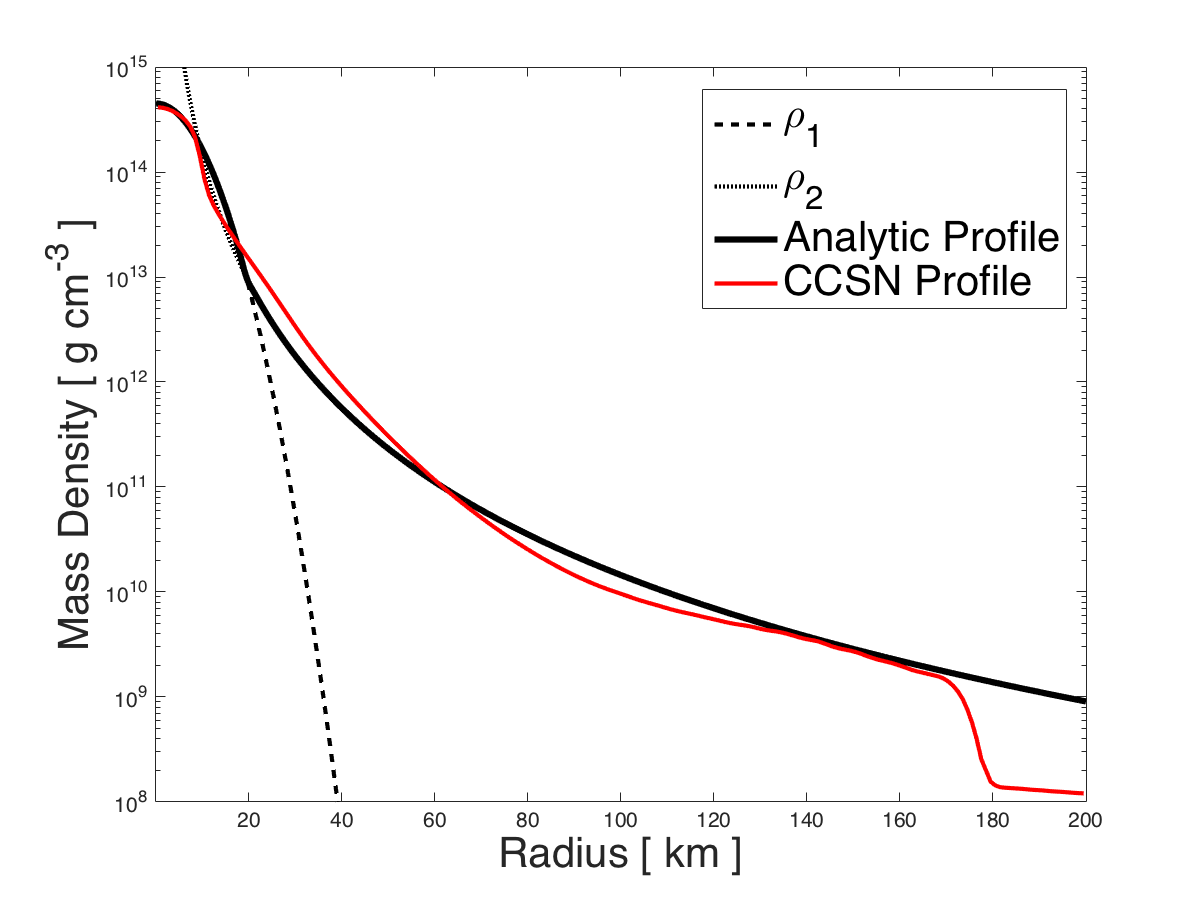
\includegraphics[scale=0.78]{./Figures/AnalyticDensityProfile}
  \end{center}
  \caption{Density profile used in the deleptonization problem (solid black line; cf. Eq.~\eqref{eq:densityProfile}).  
  It is composed of a Gaussian profile for radii $\lesssim20$~km (dashed black line), and a power law, with $\rho\propto r^{-4}$, for larger radii (dotted black line).  
  The density profile from a full physics core-collapse supernova simulation at $100$~ms after core bounce is also plotted (solid red line).  }
  \label{fig:analyticDensityProfile}
\end{figure}

\bibliographystyle{apj}
\bibliography{../References/references.bib}

\appendix

\clearpage

\section{Eigenvalues and Eigenvectors for the Two-Moment Model}
\label{sec:eigenstructure}

Here we list eigenvalues and eigenvectors for the flux Jacobian associated with the hyperbolic system in Eq.~\eqref{eq:momentEquationsCompact}.  
To this end, we define the Eddington tensor
\begin{equation}
  k^{i}_{~j}=\cK^{i}_{~j}/\cJ,
\end{equation}
where $\cK^{i}_{~j}$ is given by Eq.~\eqref{eq:stressTensor}.  

The flux Jacobian is given by
\begin{equation}
  \pderiv{\bcF^{i}(\bcM)}{\bcM}
  =\left[
  \begin{array}{cccc}
    0 & \gamma^{i1} & \gamma^{i2} & \gamma^{i3} \\
    k^{i}_{~1}+\cJ\,\pderiv{k^{i}_{~1}}{\cJ} & \cJ\,\pderiv{k^{i}_{~1}}{\cH_{1}} & \cJ\,\pderiv{k^{i}_{~1}}{\cH_{2}} & \cJ\,\pderiv{k^{i}_{~1}}{\cH_{3}} \\
    k^{i}_{~2}+\cJ\,\pderiv{k^{i}_{~2}}{\cJ} & \cJ\,\pderiv{k^{i}_{~2}}{\cH_{1}} & \cJ\,\pderiv{k^{i}_{~2}}{\cH_{2}} & \cJ\,\pderiv{k^{i}_{~2}}{\cH_{3}} \\
    k^{i}_{~3}+\cJ\,\pderiv{k^{i}_{~3}}{\cJ} & \cJ\,\pderiv{k^{i}_{~3}}{\cH_{1}} & \cJ\,\pderiv{k^{i}_{~3}}{\cH_{2}} & \cJ\,\pderiv{k^{i}_{~3}}{\cH_{3}}
  \end{array}
  \right].  
\end{equation}
We will need the derivatives
\begin{equation}
  \pderiv{\psi}{\cJ}=-\f{\cH}{\cJ^{2}}\pderiv{\psi}{h},
  \quad
  \pderiv{\psi}{\cH_{k}}=\f{h^{k}}{\cJ}\pderiv{\psi}{h},
  \quad
  \pderiv{h^{i}}{\cH_{k}}
  =\f{1}{\cH}\big(\,\gamma^{ik}-h^{i}\,h^{k}\,\big),
  \quad\text{and}\quad
  \pderiv{h_{j}}{\cH_{k}}
  =\f{1}{\cH}\big(\,\delta^{k}_{~j}-h^{k}\,h_{j}\,\big).
\end{equation}
Then, we have
\begin{equation}
  \cJ\,\pderiv{k^{i}_{~j}}{\cJ}
  =\f{1}{2}\,\big[\,\delta^{i}_{~j}-3\,h^{i}\,h_{j}\,\big]\,h\,\pderiv{\psi}{h},
\end{equation}
and
\begin{equation}
  \cJ\,\pderiv{k^{i}_{~j}}{\cH_{k}}
  =-\f{1}{2}\,\big[\,\delta^{i}_{~j}-3\,h^{i}\,h_{j}\,\big]\,h^{k}\,\pderiv{\psi}{h}
  +\f{1}{2}(3\psi-1)\,\big[\,\big(\gamma^{ik}\,h_{j}+h^{i}\,\delta^{k}_{~j}\big)-2\,h^{i}\,h^{k}\,h_{j}\,\big]\,\f{1}{h}.  
\end{equation}

Computing the flux Jacobian in the $1$-dimension, using the metric tensor in Eq.~\eqref{eq:threeMetric} and simplifying by setting $h^{2},h^{3}=0$ so that $h^{1}h_{1}=1$, gives
\begin{equation}
  \pderiv{\bcF^{1}(\bcM)}{\bcM}
  =\left[
  \begin{array}{cccc}
    0 & 1 & 0 & 0 \\
    \psi-h\,\psi' & h^{1}\,\psi' & 0 & 0 \\
    0 & 0 & \f{(3\,\psi-1)\,h^{1}}{2\,h} & 0 \\
    0 & 0 & 0 & \f{(3\,\psi-1)\,h^{1}}{2\,h}
  \end{array}
  \right],
\end{equation}
where $\psi'=\partial\psi/\partial h$.  
The characteristic polynomial is
\begin{equation}
  p(\lambda)=\Big[\,\lambda^{2}-h^{1}\,\psi'\,\lambda-\big(\,\psi-h\,\psi\,\big)\Big]\,\Big[\,\f{(3\,\psi-1)\,h^{1}}{2\,h}-\lambda\,\Big]^{2}
\end{equation}
so that the eigenvalues are
\begin{equation}
  \vect{\lambda}
  =\{\,\lambda_{1},\,\lambda_{2},\,\lambda_{3},\,\lambda_{4}\,\}
  =\big\{\,\f{1}{2}\,\big(h^{1}\,\psi'+\sqrt{\Delta}\big),\,\f{1}{2}\,\big(h^{1}\,\psi'-\sqrt{\Delta}\big),\,\f{(3\,\psi-1)\,h^{1}}{2\,h},\,\f{(3\,\psi-1)\,h^{1}}{2\,h}\,\big\},
\end{equation}
where $\Delta=(\psi'-2\,h)^{2}+4(\psi-h^{2})$ \citep[cf.][]{pons_etal_2000}.  
With the Eddington factor in Eq.~\eqref{eq:eddingtonFactor}, we have
\begin{equation}
  \psi'(h)=2\,h\,\big(\,2-h+4\,h^{2}\,\big)/5.  
\end{equation}
We then have, as expected, $\vect{\lambda}(h=0)=\{\,\sqrt{1/3},\,-\sqrt{1/3},\,0,\,0\,\}$ (diffusion limit) and $\vect{\lambda}(h=1)=\{\,h^{1},\,h^{1},\,h^{1},\,h^{1}\,\}$ (streaming limit).  

The corresponding right and left eigenvectors are given by the columns and rows, respectively of the matrices
\begin{equation}
  \cR^{1}
  =\left[
  \begin{array}{cccc}
    1 & 1 & 0 & 0 \\
    \lambda_{1} & \lambda_{2} & 0 & 0 \\
    0 & 0 & 1 & 0 \\
    0 & 0 & 0 & 1
  \end{array}
  \right]
  \quad\text{and}\quad
  \cL^{1}=(\cR^{1})^{-1}
  =\left[
  \begin{array}{cccc}
  \lambda_{2}/(\lambda_{2}-\lambda_{1}) & 1/(\lambda_{1}-\lambda_{2}) & 0 & 0 \\
  \lambda_{1}/(\lambda_{1}-\lambda_{2}) & 1/(\lambda_{2}-\lambda_{1}) & 0 & 0 \\
  0 & 0 & 1 & 0 \\
  0 & 0 & 0 & 1
  \end{array}
  \right].  
\end{equation}

\clearpage

\section{Moment Equations in Commonly Used Coordinate Systems}
\label{app:CurvilinearEuler}

\subsection{Cylindrical Coordinates}

Number conservation equation
\begin{equation}
  \pderiv{\cJ}{t}
  +\f{1}{R}\pderiv{}{R}\Big(R\,\cH^{1}\Big)
  +\pderiv{\cH^{2}}{z}
  +\pderiv{\cH^{3}}{\phi}=0,
\end{equation}
number flux equation ($R$-component)
\begin{equation}
  \pderiv{\cH_{1}}{t}
  +\f{1}{R}\pderiv{}{R}\Big(R\,\cK^{1}_{~1}\Big)
  +\pderiv{\cK^{2}_{~1}}{z}
  +\pderiv{\bcK^{3}_{~1}}{\phi}
  =\f{\cK^{3}_{~3}}{R},
\end{equation}
number flux equation ($z$-component)
\begin{equation}
  \pderiv{\cH_{2}}{t}
  +\f{1}{R}\pderiv{}{R}\Big(R\,\cK^{1}_{~2}\Big)
  +\pderiv{\cK^{2}_{~2}}{z}
  +\pderiv{\cK^{3}_{~3}}{\phi}=0,
\end{equation}
and the number flux equation ($\phi$-component)
\begin{equation}
  \pderiv{\cH_{3}}{t}
  +\f{1}{R}\pderiv{}{R}\Big(R\,\cK^{1}_{~3}\Big)
  +\pderiv{\cK^{2}_{~2}}{z}
  +\pderiv{\cK^{3}_{3}}{\phi}=0.
\end{equation}

\subsection{Spherical Coordinates}

Number conservation equation
\begin{equation}
  \pderiv{\cJ}{t}
  +\f{1}{r^{2}}\pderiv{}{r}\Big(r^{2}\,\cH^{1}\Big)
  +\f{1}{\sin\theta}\pderiv{}{\theta}\Big(\sin\theta\,\cH^{2}\Big)
  +\pderiv{}{\phi}\Big(\cH^{3}\Big)=0,
\end{equation}
number flux equation ($r$-component)
\begin{equation}
  \pderiv{\cH_{1}}{t}
  +\f{1}{r^{2}}\pderiv{}{r}\Big(r^{2}\,\cK^{1}_{~1}\Big)
  +\f{1}{\sin\theta}\pderiv{}{\theta}\Big(\sin\theta\,\cK^{2}_{~1}\Big)
  +\pderiv{\cK^{3}_{~1}}{\phi}
  =\big(\cK^{2}_{~2}+\cK^{3}_{~3}\big)\f{1}{r},
\end{equation}
number flux equation ($\theta$-component)
\begin{equation}
  \pderiv{\cH_{2}}{t}
  +\f{1}{r^{2}}\pderiv{}{r}\Big(r^{2}\,\cK^{1}_{~2}\Big)
  +\f{1}{\sin\theta}\pderiv{}{\theta}\Big(\sin\theta\,\cK^{2}_{~2}\Big)
  +\pderiv{\cK^{3}_{~2}}{\phi}
  =\cK^{3}_{~3}\cot\theta,
\end{equation}
number flux equation ($\phi$-component)
\begin{equation}
  \pderiv{\cH_{3}}{t}
  +\f{1}{r^{2}}\pderiv{}{r}\Big(\,r^{2}\,\cK^{1}_{~3}\,\Big)
  +\f{1}{\sin\theta}\pderiv{}{\theta}\Big(\sin\theta\,\cK^{2}_{~3}\,\Big)
  +\pderiv{\cK^{3}_{~3}}{\phi}=0.
\end{equation}

\end{document}
